% !TeX program = xelatex
% Compile với XeLaTeX (Overleaf: Menu > Compiler > XeLaTeX)
% BẢN RÚT GỌN 45 PHÚT (41 slide) — copy & tinh chỉnh từ bộ slide gốc 190 slide trong ../ (KHÔNG xoá bản gốc)
\documentclass[aspectratio=169,9pt]{beamer}

\usepackage{fontspec}
\setmainfont{Noto Serif}
\setsansfont{Noto Sans}
\usepackage{polyglossia}
\setmainlanguage{vietnamese}

\usepackage{amsmath,amssymb}
\usepackage{graphicx}
\usepackage{booktabs}
\usepackage{tikz}
\usetikzlibrary{arrows.meta,positioning,shapes,fit}
\usepackage{caption}
\captionsetup{font=scriptsize,labelfont=bf}
\usepackage{etoolbox}
\AtBeginEnvironment{itemize}{\setlength{\itemsep}{1pt}\setlength{\parskip}{0pt}\setlength{\topsep}{1pt}}
\AtBeginEnvironment{enumerate}{\setlength{\itemsep}{1pt}\setlength{\parskip}{0pt}\setlength{\topsep}{1pt}}
\setlength{\abovedisplayskip}{4pt}
\setlength{\belowdisplayskip}{4pt}
\setlength{\abovedisplayshortskip}{2pt}
\setlength{\belowdisplayshortskip}{2pt}

\usetheme{Madrid}
\usecolortheme{seahorse}
\setbeamertemplate{navigation symbols}{}
\setbeamertemplate{footline}[frame number]
\setbeamerfont{footnote}{size=\tiny}
\setbeamerfont{section in toc}{size=\tiny}
\setbeamerfont{subsection in toc}{size=\tiny}

\title[FastGS-lite: 3DGS \& Tăng tốc (45 phút)]{Quy trình Render 3D Gaussian Splatting\\và Cải tiến FastGS (FastGS-lite)}
\subtitle{Bản rút gọn 45 phút — Từ nền tảng đến Adaptive Density Control}
\author{Digital Twin GS}
\date{\today}

% Thư mục ảnh vẫn trỏ về figures/ gốc (Slides67/figures), vì file này nằm trong Slides67/Slides45min/
\graphicspath{{../figures/}{../../BOOK/fastergs_merge_figures/}{../../BOOK/adc_figures/}}

\begin{document}

% Lưu ý: KHÔNG đặt \titlepage ở đây — Slide 1 (trang bìa) đã nằm sẵn
% trong part45_01.tex để tránh trùng lặp trang bìa.

% ===================== 41 SLIDE RÚT GỌN, CHIA 10 FILE CHO 10 BOT =====================
% part45_01.tex : Slide 1-4   (Bìa/agenda, Động lực, 3D Gaussian là gì)
% part45_02.tex : Slide 5-8   (Hiệp phương sai, Màu SH, Pipeline render, EWA splatting)
% part45_03.tex : Slide 9-12  (Compact Box, Alpha blending, Tổng kết render, Loss)
% part45_04.tex : Slide 13-16 (Gradient biên, Tổng kết training loop, ADC tổng quan, Tích luỹ gradient)
% part45_05.tex : Slide 17-20 (Gradient cancellation, Clone, Split, Prune multi-view)
% part45_06.tex : Slide 21-24 (Reset opacity, Importance counts, Importance score, Sơ đồ densify)
% part45_07.tex : Slide 25-28 (Top-k vs Multinomial, Toy model, So sánh ADC, Kết quả 3 kịch bản)
% part45_08.tex : Slide 29-32 (Tổng kết 5 cải tiến, Vì sao 3DGS chậm, 3 đòn bẩy, Thác nước)
% part45_09.tex : Slide 33-37 (Tổng kết 3DGS→FastGS, Colab T4, Bảng 1, Bảng 3, Giới hạn phép đo)
% part45_10.tex : Slide 38-41 (RAM vs VRAM, Tổng kết pipeline, Tổng kết cải tiến, Cảm ơn/Q&A)

% ===================== part45_01.tex : Slide 1-4 =====================
% Bìa / Agenda / Động lực / 3D Gaussian là gì (rút gọn từ part1.tex, bản 45 phút)

% --- Slide 1: Trang bìa ---
\begin{frame}
\titlepage
\end{frame}

% --- Slide 2: Agenda (viết mới, rút gọn) ---
\begin{frame}{Nội dung trình bày (45 phút)}
\begin{itemize}
    \item \textbf{1.} Nền tảng: 3D Gaussian \& Spherical Harmonics (lược gọn)
    \item \textbf{2.} Chiếu phối cảnh \& Rasterizer khả vi
    \item \textbf{3.} Hàm mất mát, Gradient \& Optimizer
    \item \textbf{4.} \textbf{Trọng tâm:} Adaptive Density Control -- cải tiến đề xuất
    \item \textbf{5.} Ba đòn bẩy tăng tốc của FastGS
    \item \textbf{6.} Kết quả thực nghiệm: FastGS-lite trên Colab T4
    \item \textbf{7.} Quan sát, giới hạn \& kết luận
\end{itemize}
\vspace{0.3cm}
\small
Phần nền tảng toán học sẽ lược gọn tối đa, dành thời gian cho đóng góp chính và số liệu thực nghiệm.
\end{frame}

% --- Slide 3: Động lực: vì sao cần một biểu diễn cảnh mới? (cắt gọn từ part1.tex) ---
\begin{frame}{Động lực: vì sao cần một biểu diễn cảnh mới?}
\begin{itemize}
    \item NeRF: biểu diễn \textbf{implicit} bằng MLP, chất lượng cao nhưng render chậm (giây/khung hình) do ray-marching.
    \item 3D Gaussian Splatting (3DGS): biểu diễn \textbf{explicit} bằng hàng trăm nghìn Gaussian mờ, render bằng \textbf{rasterization khả vi}.
    \item Kết quả: hàng chục--hàng trăm FPS, gần thời gian thực.
\end{itemize}
\vspace{0.3cm}
\small
\centering
\begin{tabular}{lll}
\toprule
\textbf{Tiêu chí} & \textbf{NeRF} & \textbf{3D Gaussian Splatting} \\
\midrule
Biểu diễn & Implicit (MLP) & Explicit (tập Gaussian) \\
Render & Ray-marching, chậm & Rasterization, nhanh \\
Tốc độ & $\sim$giây/khung hình & Hàng chục--hàng trăm FPS \\
Huấn luyện & Backprop qua MLP & Backprop qua tham số Gaussian \\
\bottomrule
\end{tabular}
\end{frame}

% --- Slide 4: 3D Gaussian là gì? (cắt gọn từ part1.tex) ---
\begin{frame}{3D Gaussian là gì?}
\begin{columns}
\begin{column}{0.55\textwidth}
\footnotesize
Hàm mật độ Gaussian 3D:
\[
G(x) = \exp\left( -\frac{1}{2} (x-\mu)^T \Sigma^{-1} (x-\mu) \right)
\]
Bốn nhóm tham số học được:
\begin{itemize}
    \item Vị trí $\mu \in \mathbb{R}^3$
    \item Hiệp phương sai $\Sigma$ (hình dạng, hướng)
    \item Độ mờ (opacity) $\alpha$
    \item Màu qua hệ số Spherical Harmonics
\end{itemize}
\end{column}
\begin{column}{0.45\textwidth}
\centering
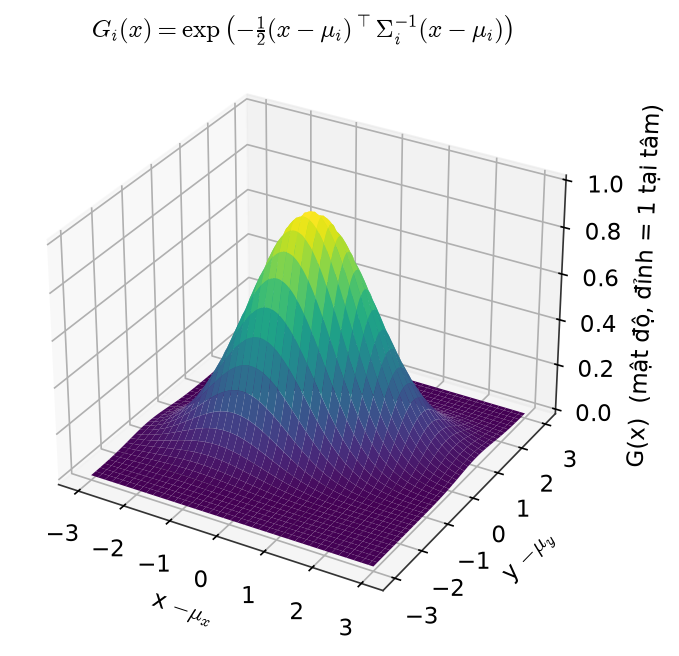
\includegraphics[width=0.95\linewidth]{ch2_gaussian_bump.png}
\captionof{figure}{\footnotesize Quả chuông mật độ Gaussian 3D}
\end{column}
\end{columns}
\end{frame}

% ============================================================
% Slide 5-8 (bản 45 phút) -- rút gọn từ part1.tex và part2.tex
% ============================================================

% --- Slide 5 (nguồn: part1.tex, "Tham số hoá hiệp phương sai") ---
\begin{frame}{Tham số hoá hiệp phương sai}
\begin{columns}
\begin{column}{0.55\textwidth}
\footnotesize
\begin{itemize}
    \item Không học trực tiếp $\Sigma$ để đảm bảo tính \textbf{positive semi-definite} khi tối ưu.
    \item Thay vào đó học scale $s \in \mathbb{R}^3$ và quaternion xoay $q \in \mathbb{R}^4$:
    \[
    \Sigma = R S S^T R^T
    \]
    với $S = \mathrm{diag}(s)$, $R = R(q)$.
\end{itemize}
\end{column}
\begin{column}{0.45\textwidth}
\centering
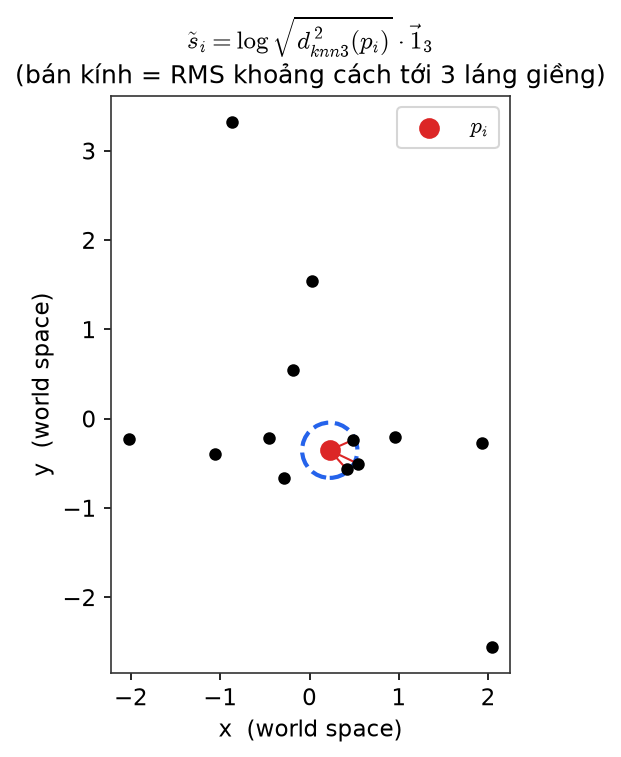
\includegraphics[width=0.78\linewidth]{ch1_scale_init.png}
\captionof{figure}{\footnotesize Khởi tạo scale từ khoảng cách lân cận}
\end{column}
\end{columns}
\end{frame}

% --- Slide 6 (nguồn: part1.tex, "Màu sắc qua Spherical Harmonics (SH)") ---
\begin{frame}{Màu sắc qua Spherical Harmonics (SH)}
\begin{columns}
\begin{column}{0.55\textwidth}
\footnotesize
\begin{itemize}
    \item Mỗi Gaussian không lưu 1 màu RGB cố định, mà lưu hệ số \textbf{SH}.
    \item Biểu diễn màu \textbf{phụ thuộc góc nhìn} (view-dependent), đặc tả hiệu ứng phản xạ/specular.
    \item Hệ số SH bậc 0 (DC) khởi tạo trực tiếp từ màu RGB quan sát được:
    \[
    f_{dc} = \mathrm{RGB2SH}(\text{color})
    \]
\end{itemize}
\end{column}
\begin{column}{0.45\textwidth}
\centering
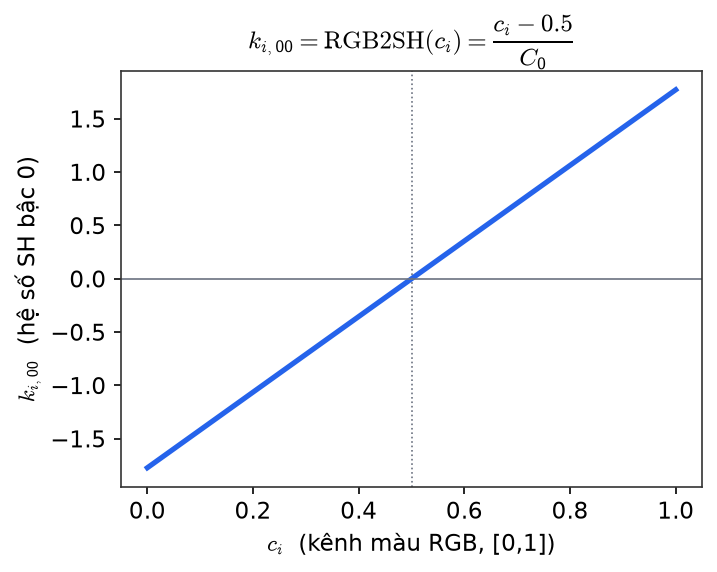
\includegraphics[width=0.95\linewidth]{ch1_rgb2sh.png}
\captionof{figure}{\footnotesize Chuyển đổi RGB $\to$ hệ số SH bậc 0}
\end{column}
\end{columns}
\vspace{0.15cm}
\footnotesize
\textit{(Phần suy diễn toán học đầy đủ của SH được trình bày chi tiết trong bản đầy đủ, không đọc trong bản 45 phút.)}
\end{frame}

% --- Slide 7 (nguồn: part2.tex, "Tổng quan pipeline render") ---
\begin{frame}{Tổng quan pipeline render}
    \begin{itemize}
        \item World $\to$ Camera: biến đổi hệ toạ độ bằng view transform $(R, t)$
        \item Projection: chiếu các Gaussian 3D xuống mặt phẳng ảnh 2D
        \item Tiling + Sorting: xác định tile ảnh hưởng và sắp theo depth
        \item Alpha blending tuần tự $\to$ màu pixel cuối cùng
    \end{itemize}
    \vspace{0.3cm}
    \centering
    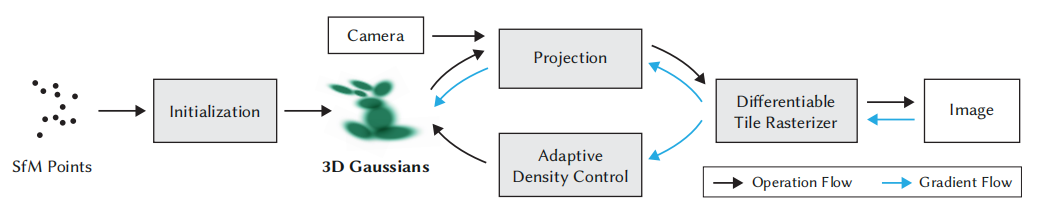
\includegraphics[width=0.95\linewidth]{pipe.png}
    \captionof{figure}{Pipeline render 3D Gaussian Splatting}
\end{frame}

% --- Slide 8 (nguồn: part2.tex, "Chiếu hiệp phương sai (EWA splatting)") ---
\begin{frame}{Chiếu hiệp phương sai (EWA splatting)}
    \begin{itemize}
        \item Phép chiếu phối cảnh phi tuyến $\to$ xấp xỉ tuyến tính cục bộ bằng Jacobian $J$ tại tâm Gaussian
        \item Hiệp phương sai 2D sau chiếu:
        \[
            \Sigma' = J\,W\,\Sigma\,W^{T}J^{T}
        \]
        trong đó $W$ là phần quay của view matrix
        \item Kỹ thuật này gọi là \textbf{Elliptical Weighted Average (EWA) splatting}
    \end{itemize}
    \vspace{0.2cm}
    \centering
    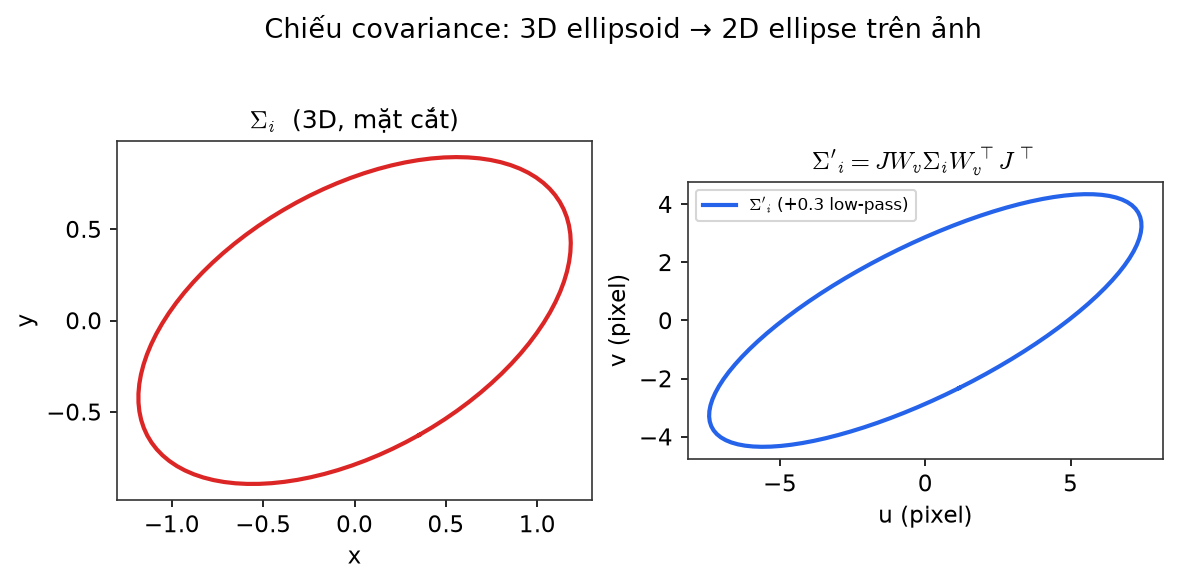
\includegraphics[width=0.6\linewidth]{ch3_ewa_projection.png}
    \captionof{figure}{Chiếu hiệp phương sai theo EWA splatting}
\end{frame}

% --- Slide 9 (từ part2.tex: Compact Box) ---
\begin{frame}{Compact Box -- đòn bẩy tăng tốc \#1 của FastGS}
\begin{columns}[T]
\begin{column}{0.52\textwidth}
\footnotesize
    \begin{itemize}
        \item Mặc định: bounding-box $3\sigma$ -- khá rộng, chạm nhiều tile không cần thiết
        \item FastGS thay bằng \textbf{compact box}: vùng ảnh hưởng 2D nhỏ hơn, điều chỉnh bằng hệ số \texttt{-{}-mult}
        \item Kết quả: giảm đáng kể số tile mỗi Gaussian phải rasterize
    \end{itemize}
\end{column}
\begin{column}{0.48\textwidth}
    \centering
    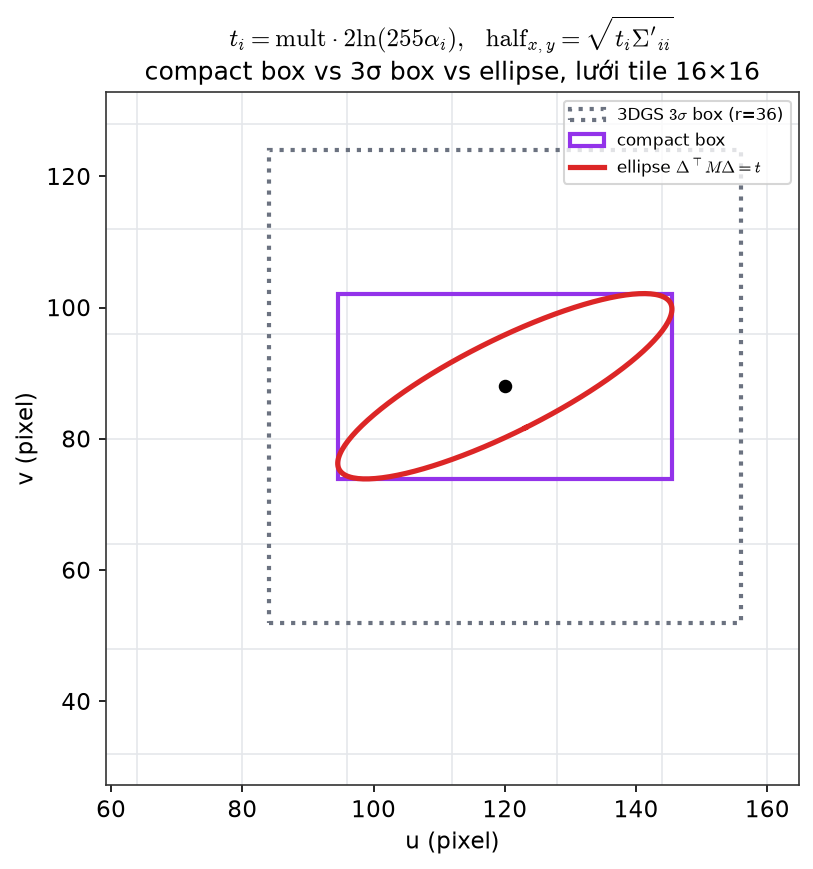
\includegraphics[width=0.95\linewidth]{ch3_compact_box.png}
    \captionof{figure}{\footnotesize So sánh bounding-box mặc định và compact box}
\end{column}
\end{columns}
\end{frame}

% --- Slide 10 (từ part2.tex: Alpha blending front-to-back) ---
\begin{frame}{Alpha blending (front-to-back)}
    \begin{itemize}
        \item Màu pixel là tổng có trọng số của các Gaussian chồng nhau theo thứ tự độ sâu
        \item Công thức blend:
        \[
            C = \sum_i c_i\,\alpha_i\,T_i, \qquad T_i = \prod_{j<i}(1-\alpha_j)
        \]
        \item $T_i$: độ truyền sáng còn lại (transmittance) trước Gaussian thứ $i$
    \end{itemize}
    \vspace{0.2cm}
    \centering
    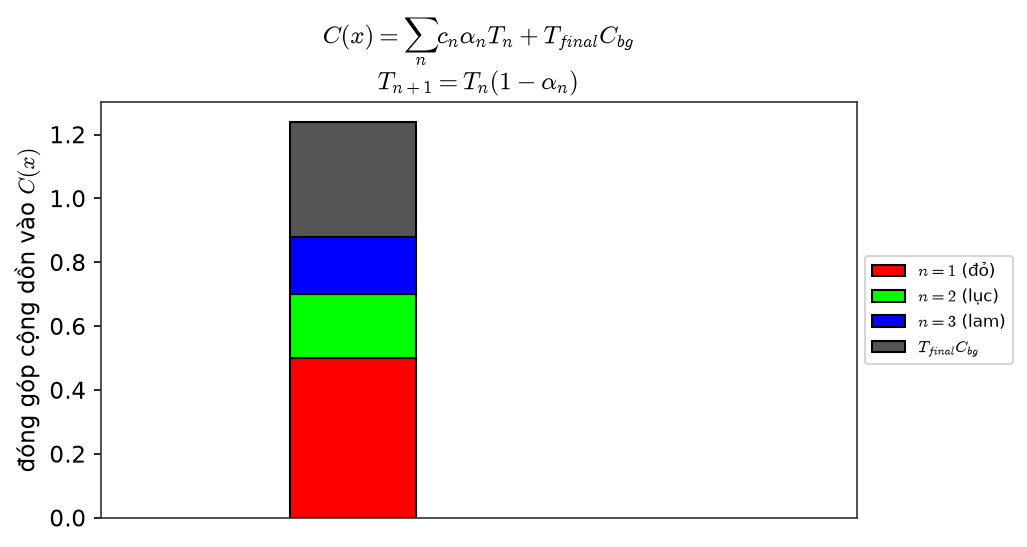
\includegraphics[width=0.55\linewidth]{ch4_alpha_blend_stack.png}
    \captionof{figure}{Chồng lớp alpha blending theo độ sâu}
\end{frame}

% --- Slide 11 (từ part2.tex: Tổng kết phương trình render) ---
\begin{frame}{Tổng kết phương trình render}
    \begin{itemize}
        \item Phương trình render đầy đủ:
        \[
            C(p) = \sum_i c_i\,\alpha_i \prod_{j<i}(1-\alpha_j)
        \]
        \item Khả vi theo mọi tham số: vị trí $\mu$, hiệp phương sai $\Sigma$, độ mờ $\alpha$, hệ số SH
    \end{itemize}
    \vspace{0.4cm}
    \centering
    \begin{tikzpicture}[node distance=1.1cm, every node/.style={font=\footnotesize}]
        \node (g3d) {Gaussian 3D};
        \node (proj) [right=of g3d] {Chiếu 2D};
        \node (alpha) [right=of proj] {Trường alpha};
        \node (blend) [right=of alpha] {Blend};
        \node (pixel) [right=of blend] {Pixel};
        \draw[-Latex] (g3d) -- (proj);
        \draw[-Latex] (proj) -- (alpha);
        \draw[-Latex] (alpha) -- (blend);
        \draw[-Latex] (blend) -- (pixel);
    \end{tikzpicture}
\end{frame}

% --- Slide 12 (từ part3.tex: Hàm mất mát L1 + D-SSIM) ---
\begin{frame}{Hàm mất mát: kết hợp L1 và D-SSIM}
    \begin{columns}[T]
        \begin{column}{0.5\textwidth}
            \begin{itemize}
                \item Loss huấn luyện kết hợp hai thành phần bổ trợ nhau:
                \begin{itemize}
                    \item \textbf{L1}: sai khác trung bình theo từng pixel.
                    \item \textbf{D-SSIM}: $1-\text{SSIM}$, phản ánh sai lệch \textbf{cấu trúc}.
                \end{itemize}
                \item Công thức tổng:
                \[
                    \mathcal{L} = (1-\lambda)\,\mathcal{L}_1 + \lambda\,(1-\text{SSIM})
                \]
                \item Hệ số $\lambda = $ \texttt{lambda\_dssim}: mặc định $0.2$, \texttt{fastgs-lite}: $0.25$
            \end{itemize}
        \end{column}
        \begin{column}{0.5\textwidth}
            \centering
            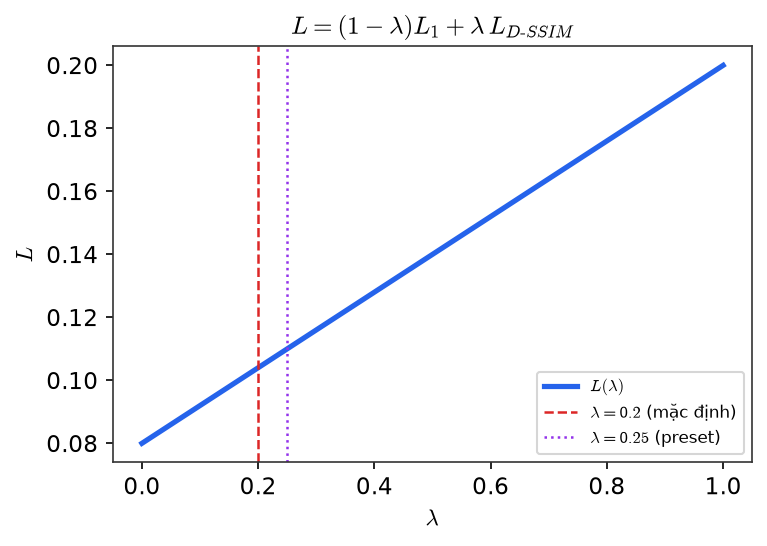
\includegraphics[width=0.95\linewidth]{ch5_loss_mix.png}
            \captionof{figure}{Tỉ trọng L1 và D-SSIM trong loss}
        \end{column}
    \end{columns}
\end{frame}

% ============================================================
% Slide 13-16 (bản 45 phút) -- rút gọn từ part3.tex, part4.tex
% ============================================================

% --- Slide 13 (part3.tex: Gradient tập trung tại biên Gaussian) ---
\begin{frame}{Gradient tập trung tại biên Gaussian}
    \begin{columns}[T]
        \begin{column}{0.5\textwidth}
            \begin{itemize}
                \item Gradient view-space lớn nhất xuất hiện ở vùng \textbf{biên/rìa} của Gaussian -- nơi ảnh render lệch nhiều nhất so với ảnh thật.
                \item Gradient tại biên chính là \textbf{tín hiệu} quyết định \textbf{densify} (thêm Gaussian mới) ở giai đoạn sau.
                \item Vùng gradient thấp $\Rightarrow$ Gaussian đã khớp tốt, không cần chia tách thêm.
            \end{itemize}
        \end{column}
        \begin{column}{0.5\textwidth}
            \centering
            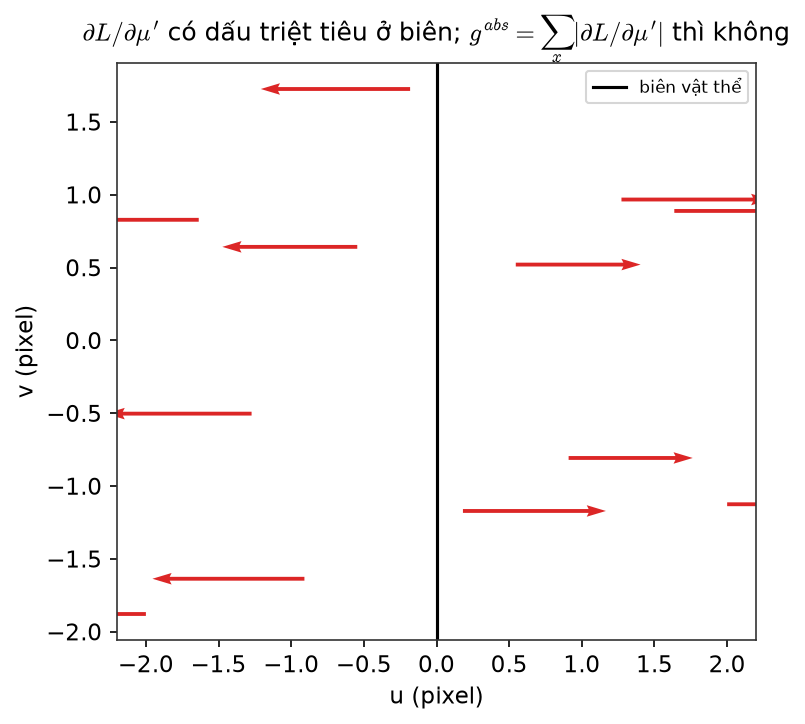
\includegraphics[width=0.95\linewidth]{ch6_edge_gradient.png}
            \captionof{figure}{Gradient tập trung ở biên Gaussian}
        \end{column}
    \end{columns}
\end{frame}

% --- Slide 14 (part3.tex: Tổng kết vòng lặp huấn luyện) ---
\begin{frame}{Tổng kết vòng lặp huấn luyện}
    \begin{center}
        \footnotesize
        \begin{tikzpicture}[
            node distance=1.1cm and 1.6cm,
            box/.style={draw, rounded corners, fill=blue!8, align=center, minimum width=2.6cm, minimum height=1cm},
            ->, thick
        ]
            \node[box] (render) {1. Render};
            \node[box, right=of render] (loss) {2. Tính loss\\ (L1 + D-SSIM)};
            \node[box, right=of loss] (backward) {3. Backward\\ (lan gradient)};
            \node[box, below=of loss] (step) {4. optimizer.step()\\ (sparse Adam)};
            \node[box, left=of step] (dp) {5. Densify /\\ Prune (định kỳ)};

            \draw (render) -- (loss);
            \draw (loss) -- (backward);
            \draw (backward) |- (step);
            \draw (step) -- (dp);
            \draw (dp) |- (render);
        \end{tikzpicture}
    \end{center}
    \begin{itemize}
        \item Một iteration: \textbf{render} $\to$ \textbf{loss} $\to$ \textbf{backward} $\to$ \textbf{optimizer.step()} $\to$ (định kỳ) \textbf{densify/prune} $\to$ lặp lại đến hội tụ.
    \end{itemize}
\end{frame}

% --- Slide 15 (part4.tex: Tổng quan Adaptive Density Control (ADC)) ---
\begin{frame}{Tổng quan Adaptive Density Control (ADC)}
    \begin{itemize}
        \item Point cloud khởi tạo từ COLMAP thường \textbf{quá thưa} ở vùng thiếu chi tiết, đồng thời có Gaussian \textbf{quá to} che khuất chi tiết nhỏ.
        \item ADC chạy định kỳ mỗi \texttt{densification\_interval} iteration để điều chỉnh mật độ Gaussian:
        \begin{itemize}
            \item \textbf{Densify}: nhân bản (clone) hoặc tách (split) Gaussian thiếu hình học.
            \item \textbf{Prune}: cắt tỉa Gaussian thừa, mờ, vô dụng.
        \end{itemize}
        \item Mục tiêu: cân bằng chất lượng tái tạo và số lượng Gaussian (bộ nhớ, tốc độ render).
    \end{itemize}
    \vspace{0.2cm}
    \centering
    \begin{tikzpicture}[node distance=1.4cm, every node/.style={font=\footnotesize}]
        \node[draw, rounded corners, fill=blue!10] (adc) {ADC};
        \node[draw, rounded corners, fill=green!10, below left=0.9cm and 1.6cm of adc] (clone) {Clone};
        \node[draw, rounded corners, fill=orange!10, below=1.2cm of adc] (split) {Split};
        \node[draw, rounded corners, fill=red!10, below right=0.9cm and 1.6cm of adc] (prune) {Prune};
        \draw[->] (adc) -- (clone);
        \draw[->] (adc) -- (split);
        \draw[->] (adc) -- (prune);
    \end{tikzpicture}
\end{frame}

% --- Slide 16 (part4.tex: Tích luỹ gradient view-space) ---
\begin{frame}{Tích luỹ gradient view-space}
\begin{columns}[T]
\begin{column}{0.52\textwidth}
\footnotesize
    \begin{itemize}
        \item Với mỗi Gaussian, gradient vị trí 2D (view-space) được \textbf{cộng dồn} qua nhiều lần render từ các camera khác nhau.
        \item Đồng thời đếm \texttt{denom}: số lần Gaussian đó thực sự visible trong batch.
        \item Gradient trung bình dùng làm tín hiệu densify:
        \[
            \bar{g} = \frac{\sum_{v} \nabla_{\text{view}} }{\text{denom}}
        \]
        \item $\bar g$ lớn $\Rightarrow$ ứng viên clone/split.
    \end{itemize}
\end{column}
\begin{column}{0.48\textwidth}
    \centering
    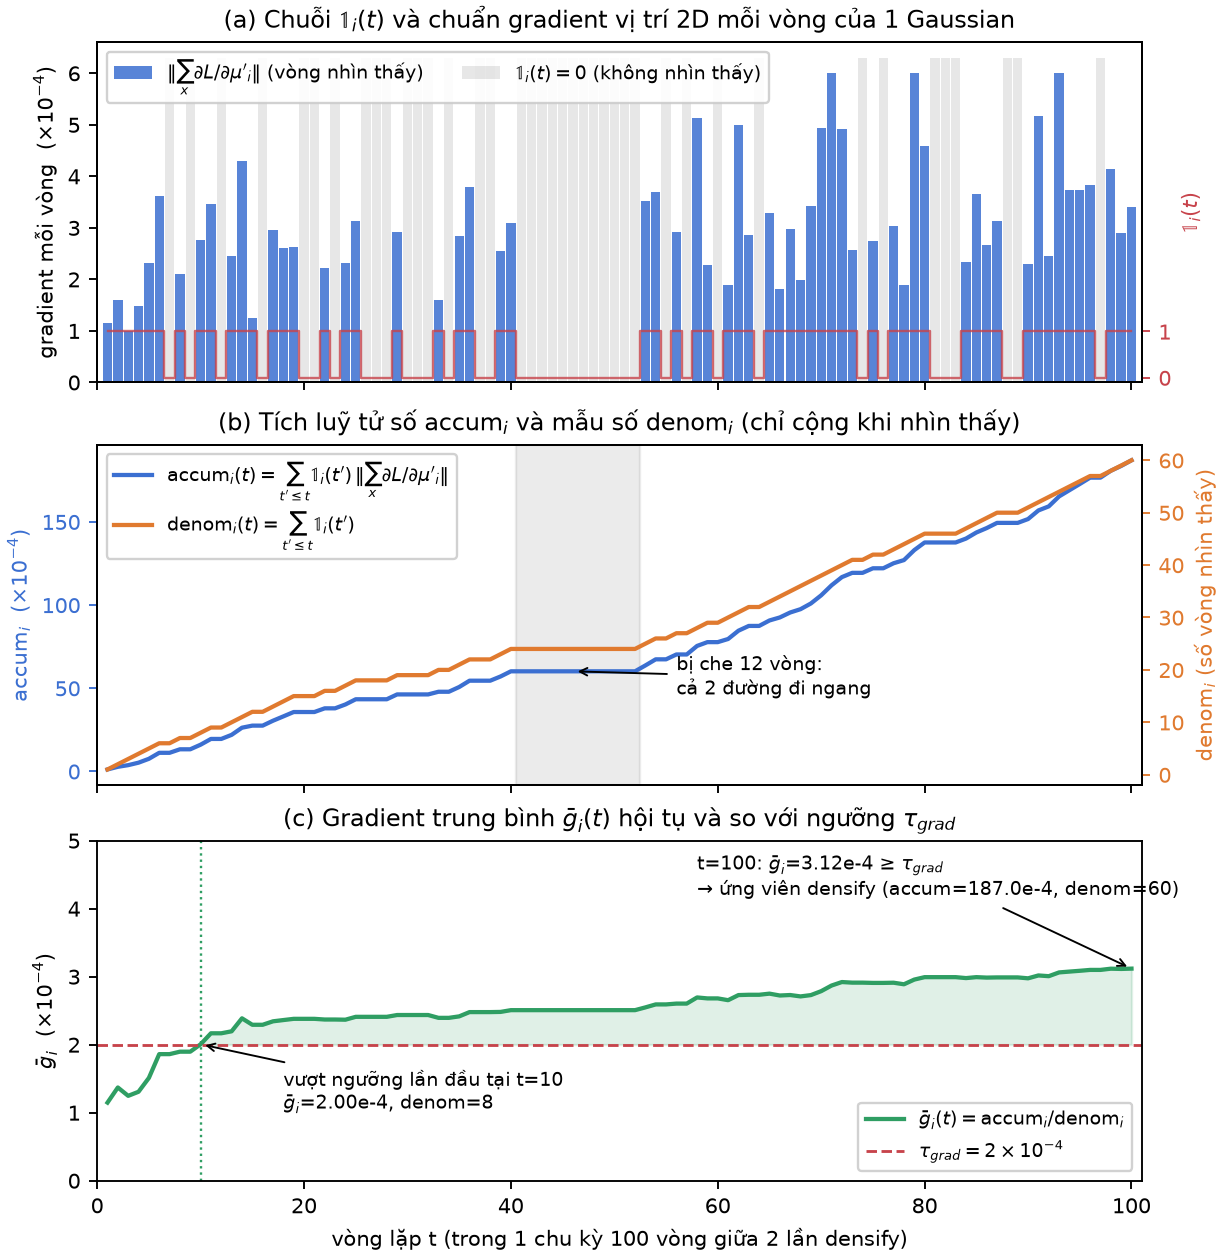
\includegraphics[width=0.95\linewidth]{fig_02_accum_denom.png}
\end{column}
\end{columns}
\end{frame}

\begin{frame}{Vấn đề triệt tiêu gradient (gradient cancellation)}
    \begin{itemize}
        \item Khi lấy trung bình vector gradient từ \textbf{nhiều view có hướng ngược nhau}, chúng có thể \textbf{triệt tiêu lẫn nhau}.
        \item Hệ quả: dù mỗi view riêng lẻ báo lỗi lớn, $\bar g$ trung bình vẫn nhỏ $\Rightarrow$ Gaussian \textbf{bị bỏ sót}, không được densify.
        \item FastGS cải thiện bằng \textbf{multi-view consistency score} thay vì chỉ dựa vào gradient trung bình.
    \end{itemize}
    \vspace{0.2cm}
    \centering
    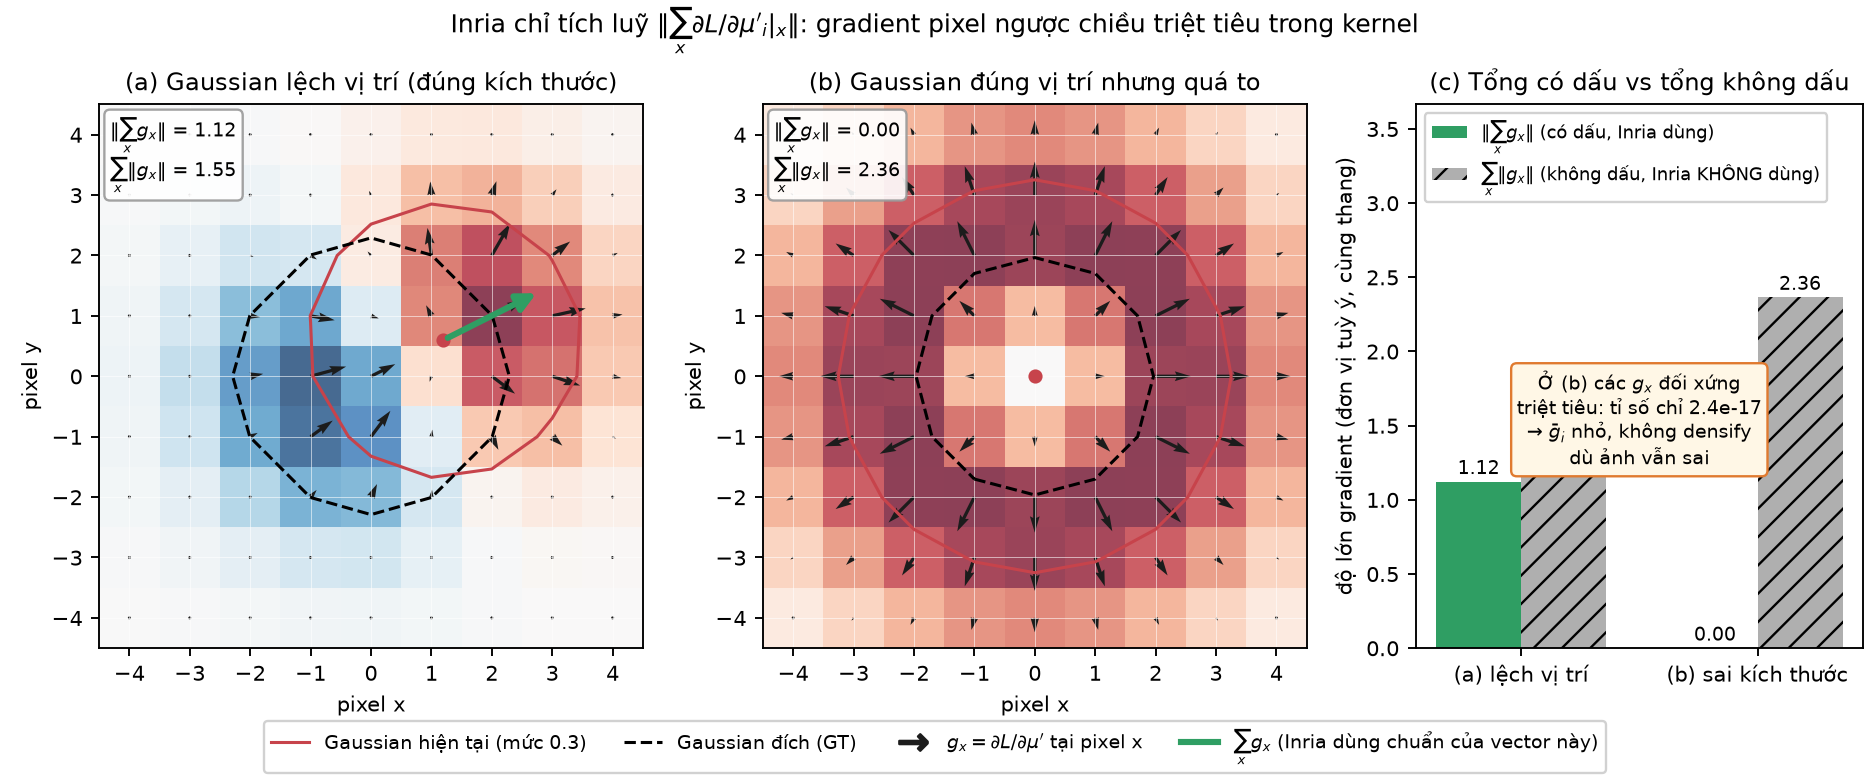
\includegraphics[width=0.7\linewidth]{fig_03_grad_cancel.png}
\end{frame}

% --- Slide 36 ---
\begin{frame}{Clone (nhân bản)}
    \footnotesize
    \begin{itemize}
        \item Áp dụng cho Gaussian \textbf{nhỏ nhưng thiếu hình học} (under-reconstruction).
        \item Nhân đôi Gaussian theo \textbf{hướng gradient vị trí} $\bar g$, đặt bản sao lệch một khoảng nhỏ.
        \item \textbf{Không} thay đổi kích thước/covariance -- chỉ lấp đầy vùng thiếu chi tiết bằng tăng mật độ.
    \end{itemize}
    \begin{columns}
        \begin{column}{0.48\linewidth}
            \centering
            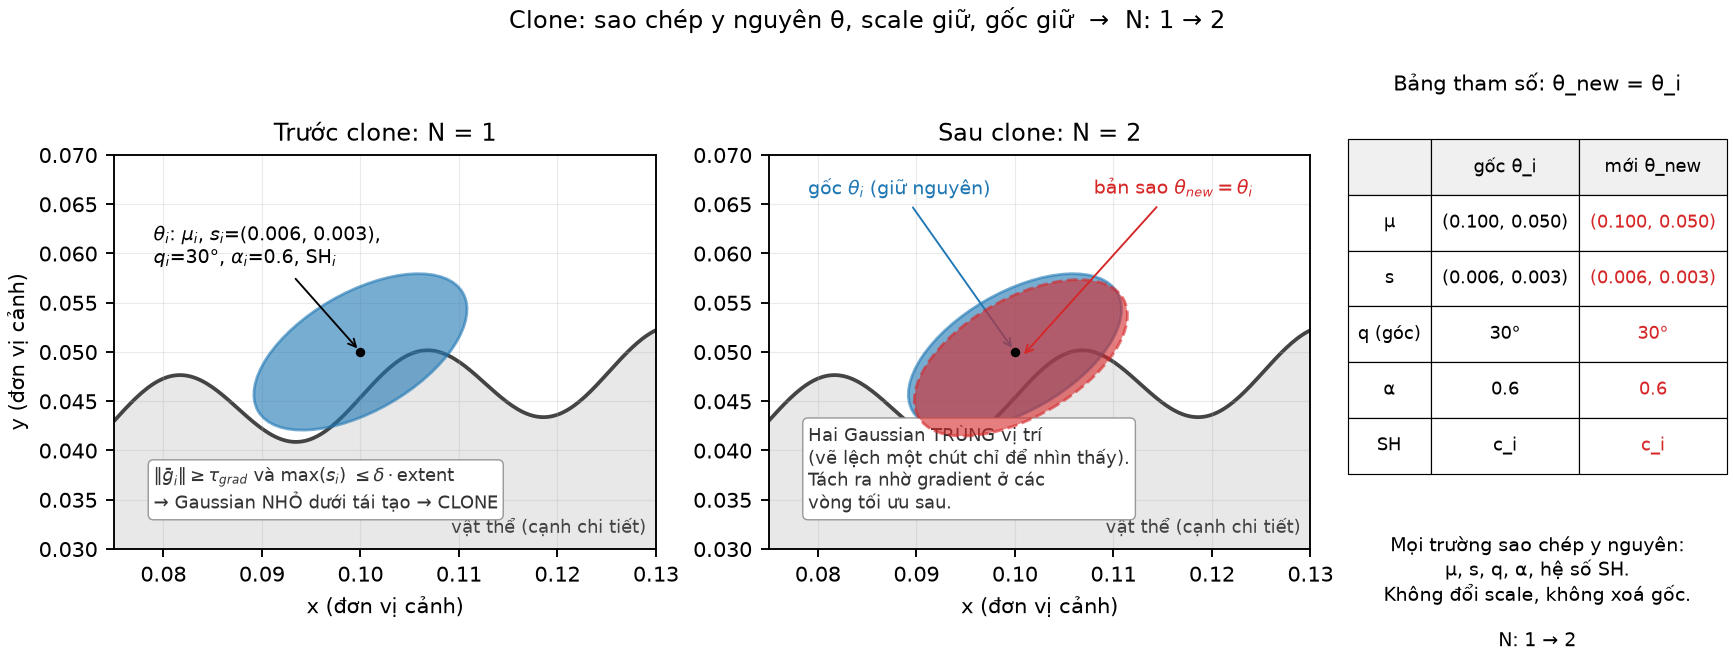
\includegraphics[width=\linewidth]{fig_08_clone_before_after.png}
            \captionof{figure}{Trước/sau clone}
        \end{column}
        \begin{column}{0.48\linewidth}
            \centering
            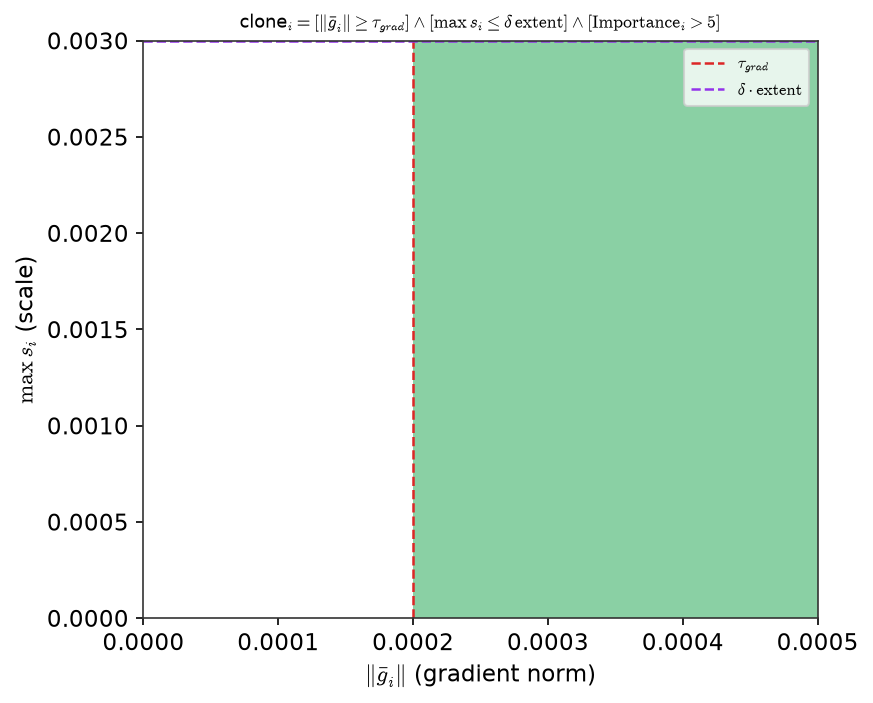
\includegraphics[width=\linewidth]{ch7_clone_region.png}
            \captionof{figure}{Vùng được clone}
        \end{column}
    \end{columns}
\end{frame}

% --- Slide 37 ---
\begin{frame}{Split (tách)}
    \footnotesize
    \begin{itemize}
        \item Áp dụng cho Gaussian \textbf{quá to} (over-reconstruction), vượt ngưỡng \texttt{--dense} theo scene extent.
        \item Tách thành \textbf{2 Gaussian con} nhỏ hơn (giảm scale theo hệ số cố định).
        \item Vị trí Gaussian con được \textbf{lấy mẫu ngẫu nhiên} theo phân phối chuẩn dựa trên covariance gốc của Gaussian cha.
    \end{itemize}
    \begin{columns}
        \begin{column}{0.48\linewidth}
            \centering
            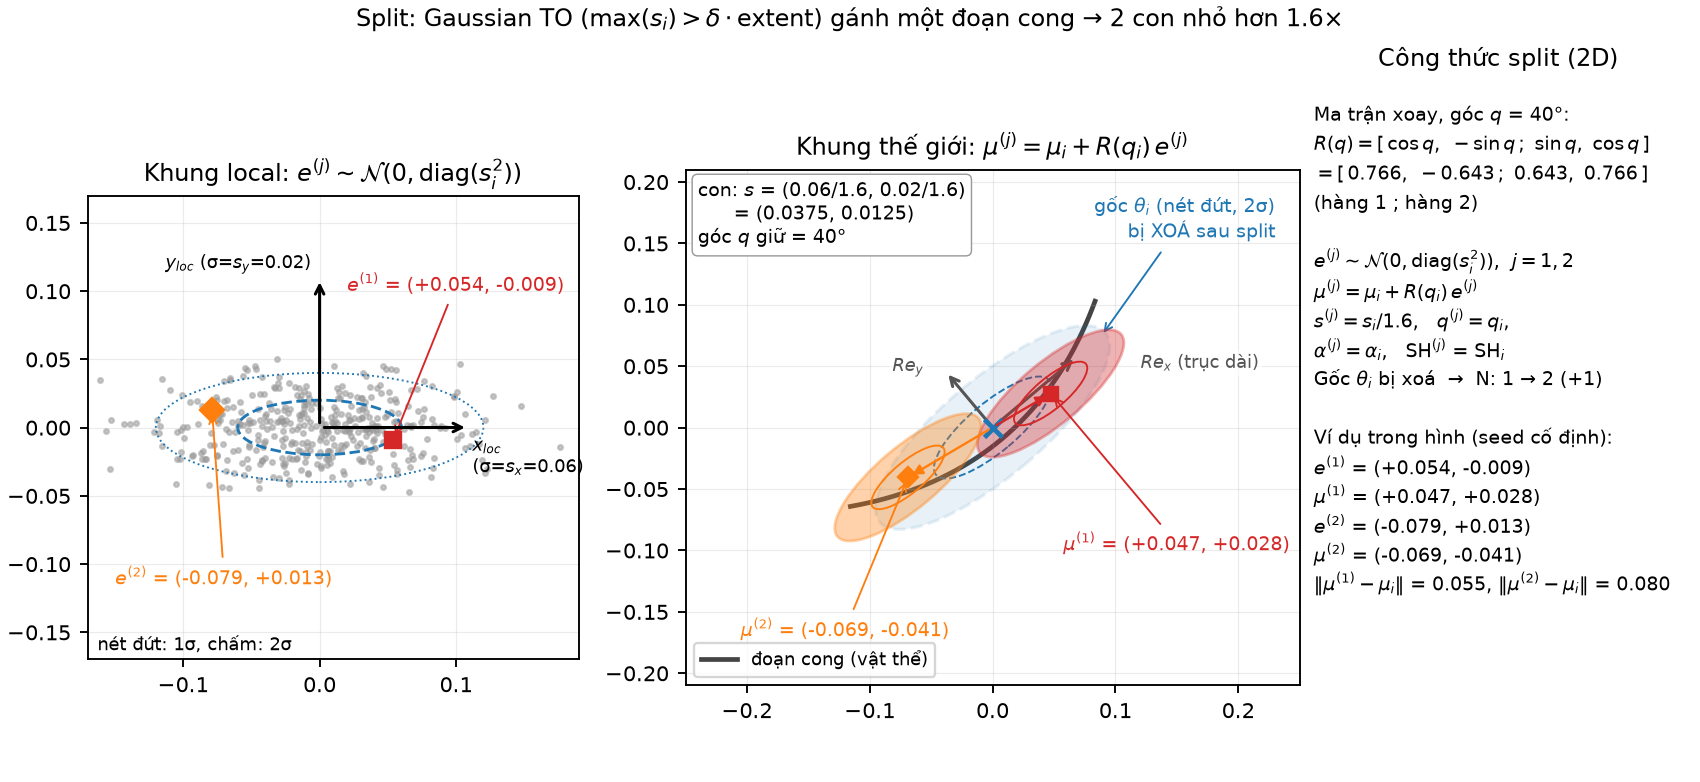
\includegraphics[width=\linewidth]{fig_09_split_geometry.png}
            \captionof{figure}{Hình học split}
        \end{column}
        \begin{column}{0.48\linewidth}
            \centering
            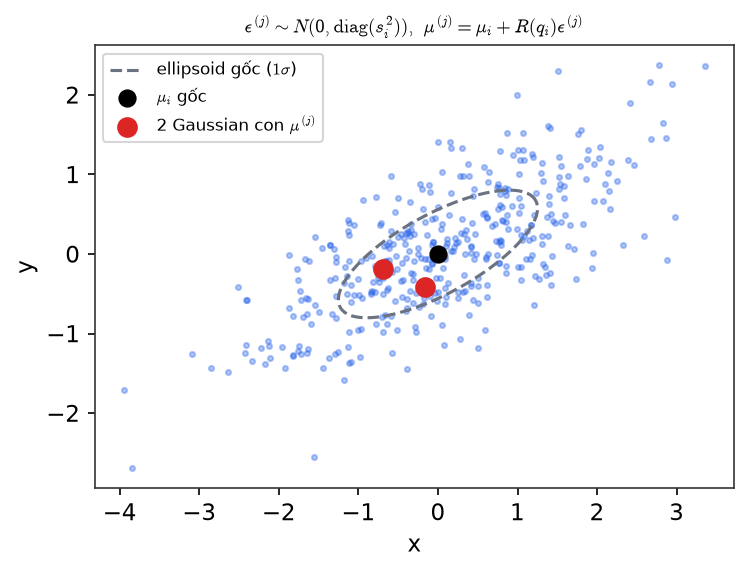
\includegraphics[width=\linewidth]{ch7_split_sampling.png}
            \captionof{figure}{Lấy mẫu theo covariance}
        \end{column}
    \end{columns}
\end{frame}

% --- Slide 38 ---
\begin{frame}{Prune theo độ quan trọng đa góc nhìn (FastGS)}
    \begin{itemize}
        \item 3DGS gốc: prune đơn thuần theo ngưỡng \textbf{opacity thấp} hoặc \textbf{kích thước quá lớn}.
        \item \textbf{FastGS}: tính điểm \emph{importance} cho mỗi Gaussian dựa trên đóng góp thực tế vào chất lượng ảnh render, tổng hợp qua \textbf{nhiều góc nhìn}.
        \item Gaussian có điểm importance thấp nhất bị cắt tỉa trước, bất kể opacity/kích thước.
        \item Kết quả: mô hình \textbf{gọn hơn} nhưng vẫn giữ chất lượng tái tạo -- đây là \textbf{đòn bẩy chính} giúp FastGS tăng tốc.
    \end{itemize}
    \vspace{0.2cm}
    \centering
    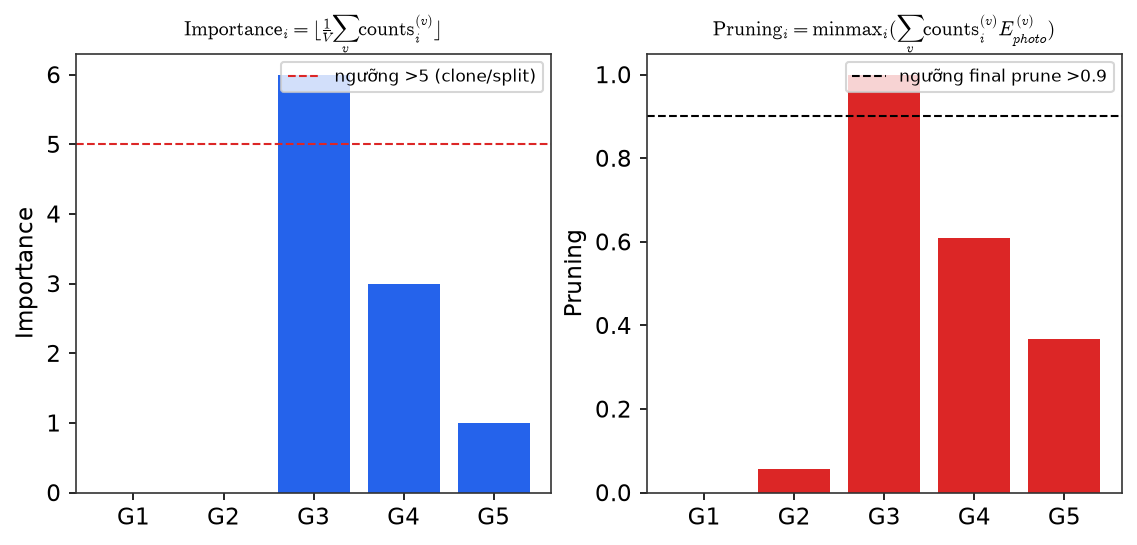
\includegraphics[width=0.7\linewidth]{ch7_importance_pruning.png}
\end{frame}

% ============================================================
% Slide 21-24 (bản 45 phút) — rút gọn từ part4.tex / partADC_2a.tex / partADC_4a.tex
% ============================================================

% --- Slide 21 (gốc: part4.tex, "Reset opacity định kỳ") ---
\begin{frame}{Reset opacity định kỳ}
    \footnotesize
    \begin{itemize}
        \item Mỗi \texttt{opacity\_reset\_interval} (mặc định 3000 iteration): toàn bộ opacity reset về \textbf{giá trị thấp} (qua sigmoid-inverse).
        \item Buộc optimizer \textbf{"đánh giá lại"} từng Gaussian từ đầu.
        \item Gaussian thực sự cần thiết: opacity \textbf{tăng trở lại}; Gaussian dư thừa: không hồi phục kịp $\Rightarrow$ bị \textbf{prune} ở vòng sau.
    \end{itemize}
    \begin{columns}
        \begin{column}{0.48\linewidth}
            \centering
            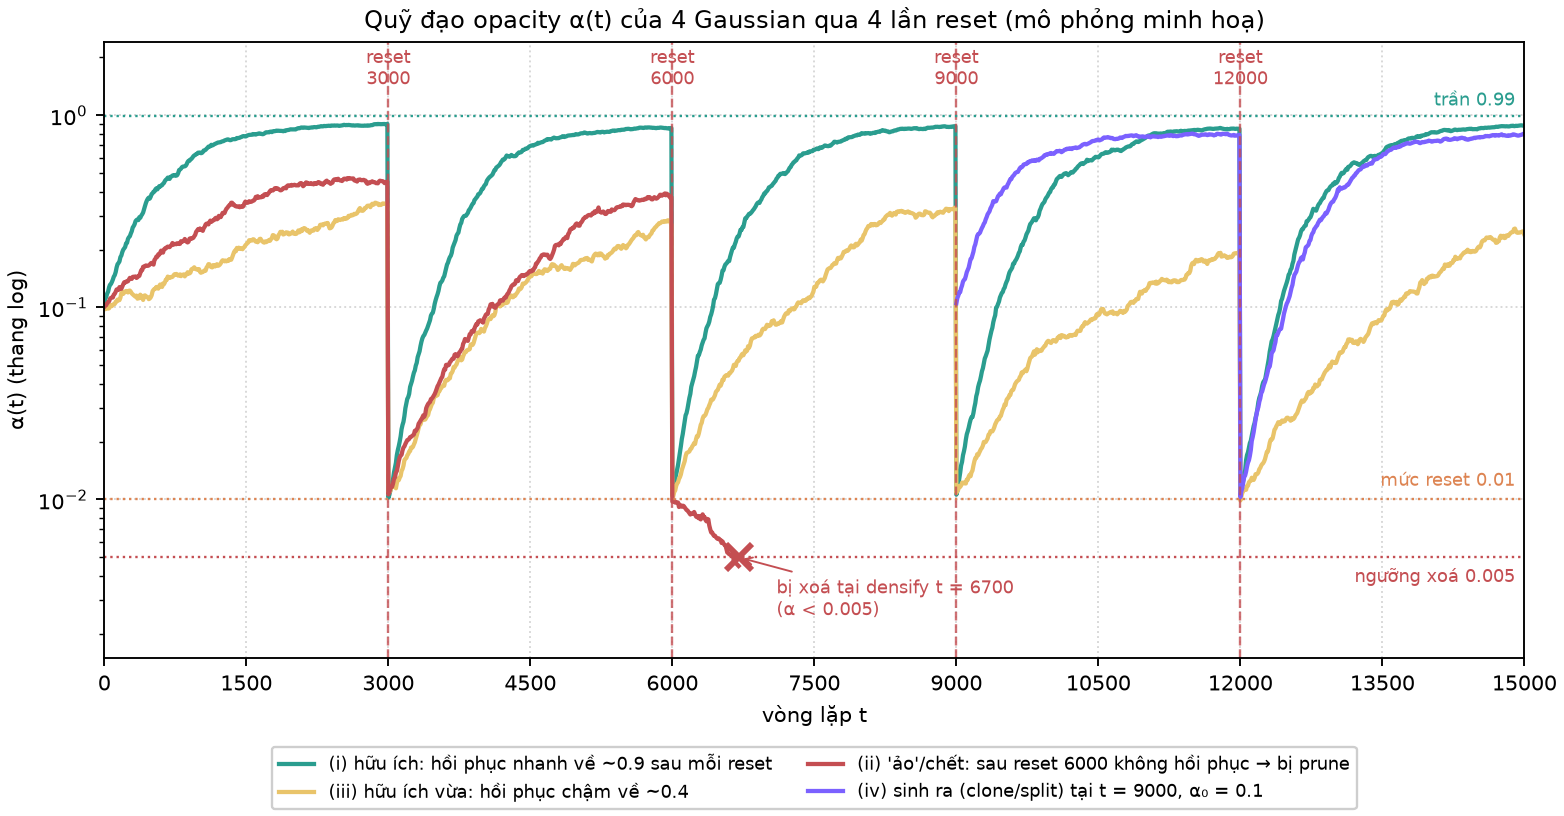
\includegraphics[width=\linewidth]{fig_17_opacity_trajectory.png}
            \captionof{figure}{Quỹ đạo opacity theo thời gian}
        \end{column}
        \begin{column}{0.48\linewidth}
            \centering
            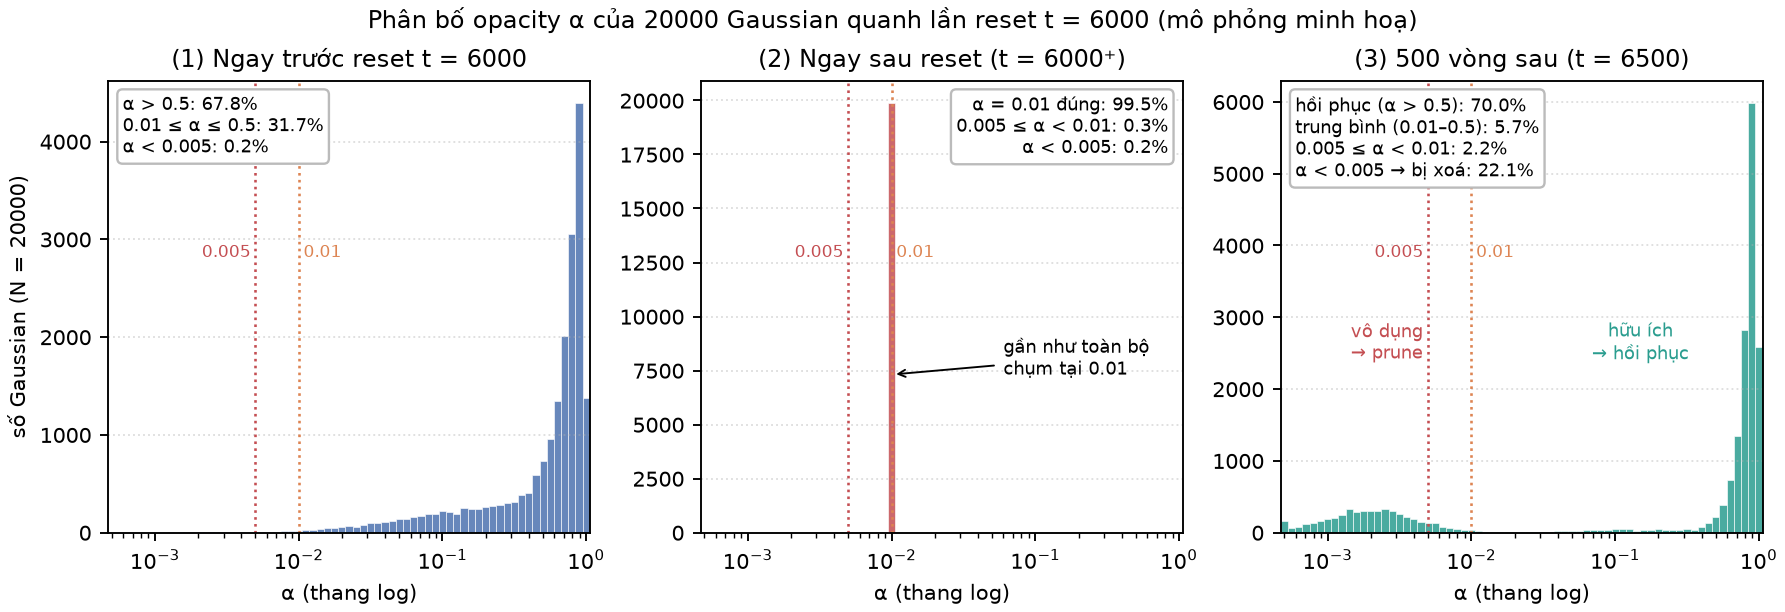
\includegraphics[width=\linewidth]{fig_18_hist_reset.png}
            \captionof{figure}{Histogram trước/sau reset}
        \end{column}
    \end{columns}
\end{frame}

% --- Slide 22 (gốc: partADC_2a.tex, "Tổng hợp counts qua nhiều view: đầu vào cho Importance") ---
\begin{frame}{Tổng hợp counts qua nhiều view: đầu vào cho Importance}
    \footnotesize
    \begin{itemize}
        \item Mỗi Gaussian $i$ có vector counts $(\text{counts}_i^1, \text{counts}_i^2, \text{counts}_i^3)$ theo từng view.
        \item Tổng số lỗi bị "tố cáo" trên mỗi view luôn $\ge$ số pixel lỗi thật:
        \[
            \sum_i \text{counts}_i^v \ \ge\ |m_v|
        \]
        vì một pixel lỗi có thể được nhiều Gaussian chồng lấn cùng đếm.
        \item Trong code: mỗi lần render view $v$, kernel CUDA cộng dồn atomic vào \texttt{metricCount}$[N]$, rồi lũy kế: \texttt{full\_metric\_counts += counts\textsuperscript{(v)}}.
        \item Vector counts tổng hợp qua $V$ view là đầu vào trực tiếp cho bước tính Importance.
    \end{itemize}
    \centering
    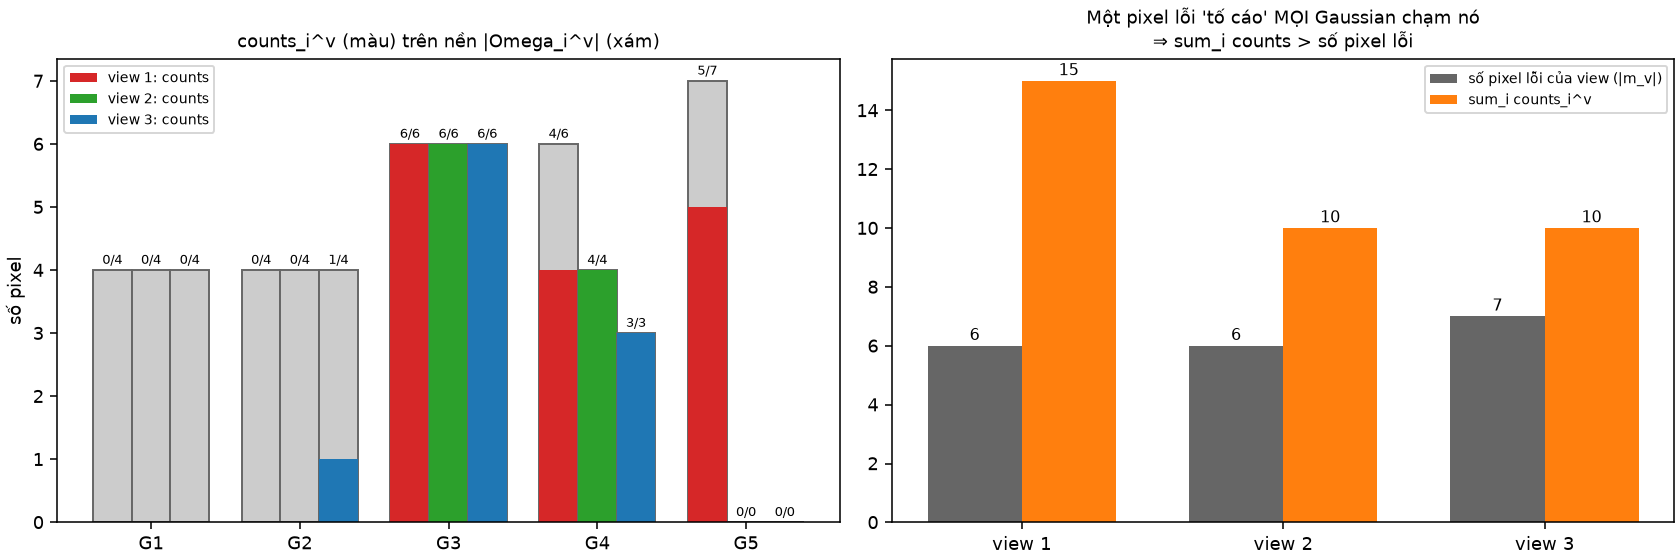
\includegraphics[width=0.85\linewidth]{2_4_bar-counts-moi-view.png}
    \captionof{figure}{\footnotesize Trái: counts$_i^v$ (màu) trên nền $|\Omega_i^v|$ (xám). Phải: $|m_v|$ so với $\sum_i \text{counts}_i^v$ mỗi view.}
\end{frame}

% --- Slide 23 (gốc: partADC_2a.tex, "Importance score: trung bình counts qua các view, làm tròn xuống") ---
\begin{frame}{Importance score: trung bình counts qua các view, làm tròn xuống}
    \footnotesize
    \begin{itemize}
        \item Công thức Importance (khớp code \texttt{compute\_gaussian\_score\_fastgs}):
        \[
            \text{Importance}_i = \left\lfloor \frac{1}{V} \sum_{v=1}^{V} \text{counts}_i^v \right\rfloor
        \]
        (\texttt{torch.div(full\_metric\_counts, V, rounding\_mode='floor')}).
        \item Gaussian được xem là "quan trọng" (giữ lại/densify) khi $\text{Importance}_i > 5$.
        \item Ví dụ $4\times4$, $3$ view: chỉ $G3$ có mean $> 5$ vượt ngưỡng; các Gaussian còn lại bị chặn.
        \item Màu nóng trong heatmap = Gaussian đóng góp nhiều vào vùng lỗi cao (giữ lại); màu lạnh = ứng viên prune.
    \end{itemize}
    \centering
    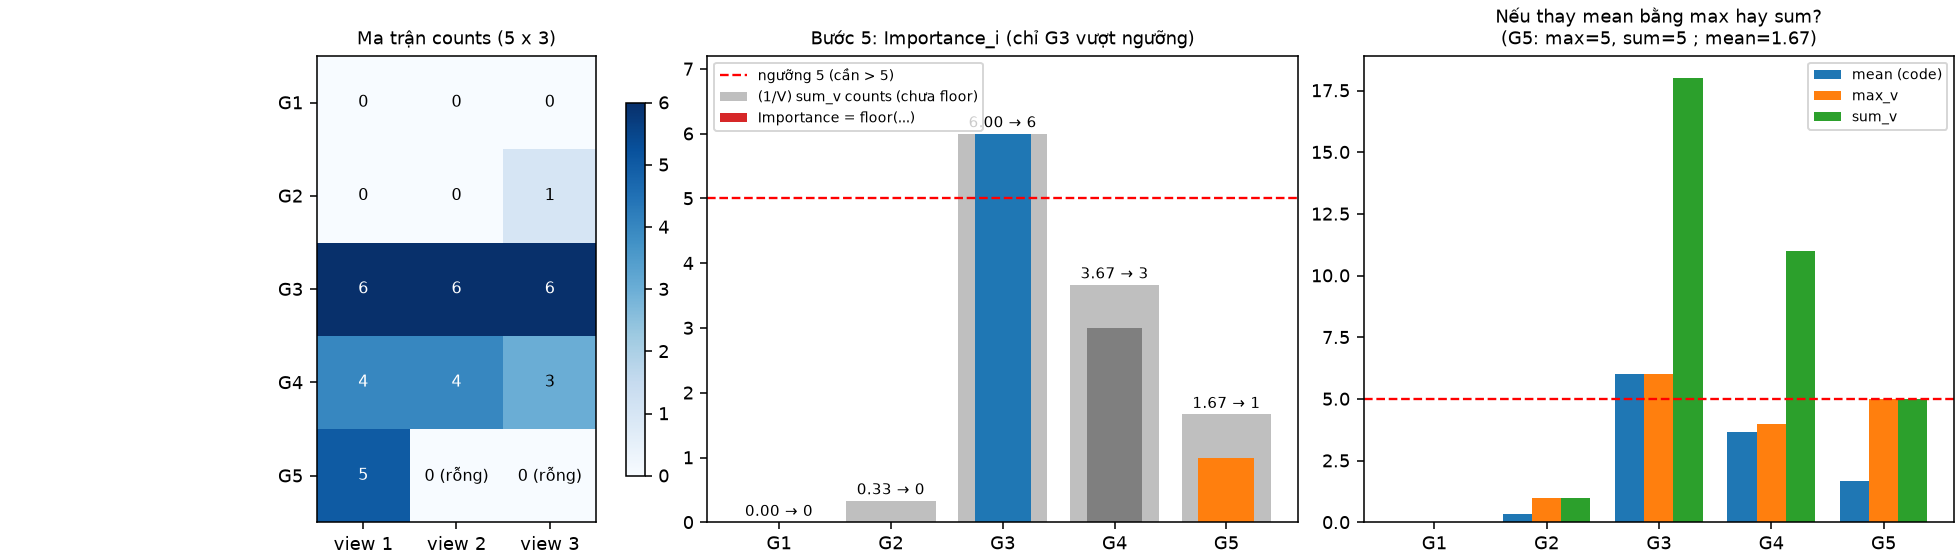
\includegraphics[width=0.85\linewidth]{2_5_importance-heatmap.png}
    \captionof{figure}{\footnotesize Trái: ma trận counts $(5\times 3)$. Giữa: Importance$_i = \lfloor \text{mean}_v \rfloor$, ngưỡng $5$. Phải: so sánh mean vs.\ max vs.\ sum.}
\end{frame}

% --- Slide 24 (gốc: partADC_4a.tex, "Sơ đồ quyết định densify đầy đủ") ---
\begin{frame}{Sơ đồ quyết định densify đầy đủ}
\begin{columns}[T]
\begin{column}{0.48\linewidth}
\footnotesize
\begin{itemize}
  \item Áp dụng cho mỗi Gaussian $i$, mỗi 100 (hoặc 500) vòng lặp, khi $500 < t < 15000$.
  \item \textbf{Bước 1 — kích thước chọn nhánh:} $\max s_i \le \delta \cdot \text{extent}\;?$
  \item \textbf{Nhánh NHỎ:} nếu $\bar g_i \ge \tau_{\text{grad}} = 2\times10^{-4}$ \textbf{và} $\text{Imp}_i > 5$ $\Rightarrow$ \textbf{CLONE} ($1 \to 2$, giữ bản gốc).
  \item \textbf{Nhánh TO:} nếu $\bar g_{\text{abs},i} \ge \tau_{\text{abs}} = 1.2\times10^{-3}$ \textbf{và} $\text{Imp}_i > 5$ $\Rightarrow$ \textbf{SPLIT} (2 con, xoá gốc, $1 \to 2$).
  \item Nếu Importance không thoả: 3DGS gốc vẫn densify, FastGS-lite thì không.
  \item Nguồn: \texttt{densify\_and\_prune\_fastgs}, \texttt{gaussian\_model.py:449-462}.
\end{itemize}
\end{column}
\begin{column}{0.5\linewidth}
\centering
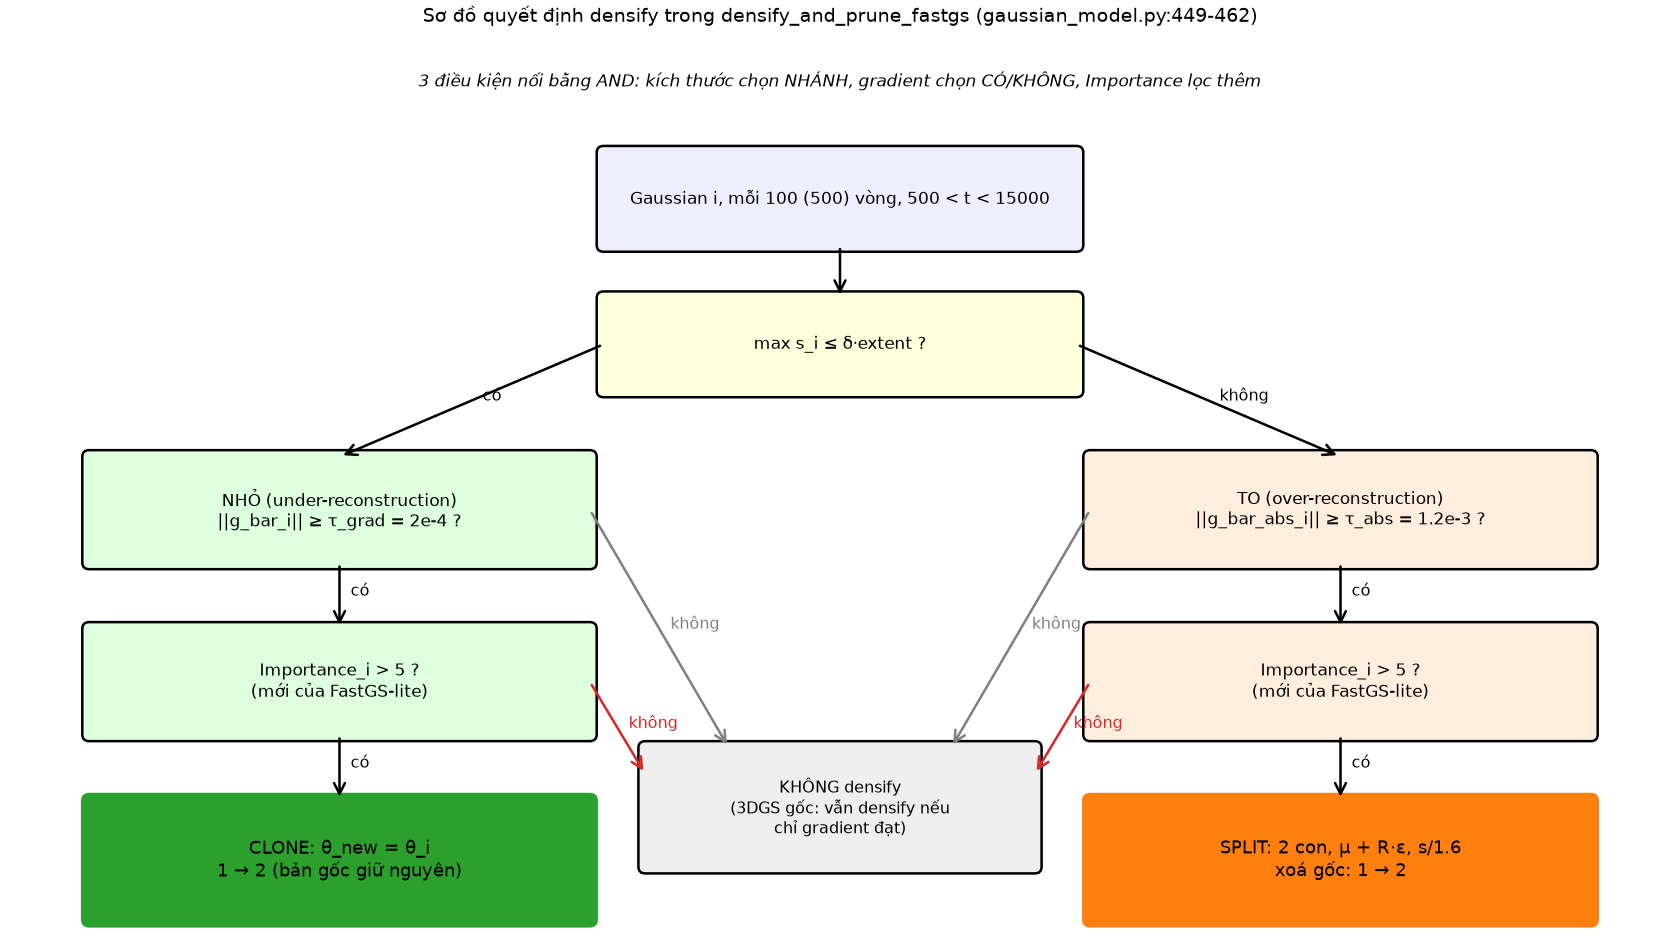
\includegraphics[width=\linewidth]{4_6_decision-diagram.png}
\captionof{figure}{\footnotesize 3 điều kiện nối bằng AND: kích thước chọn nhánh, gradient chọn có/không, Importance lọc thêm.}
\end{column}
\end{columns}
\end{frame}

% part45_07.tex — Slide 25-28 (ban rut gon 45 phut)
% Chi chua 4 khoi frame, khong documentclass/usepackage/begin{document}.
% Nguon: partADC_5a.tex, partADC_6.tex, partADC_7.tex (KHONG sua file goc).

% ===== Slide 25 (nguon: partADC_5a.tex, frame "Top-k cứng vs. Multinomial") =====
\begin{frame}{Top-k cứng vs.\ Multinomial: hai chiến lược pruning}
\begin{columns}[T]
\begin{column}{0.5\linewidth}
\footnotesize
\begin{itemize}
    \item Mô phỏng $N=300$ Gaussian, điểm số $P_i$ chuẩn hoá min--max từ \texttt{Beta}$(2{,}2{,}5)$; tập ứng viên $C$ chọn ngẫu nhiên $40\%$ quần thể, budget $=\lfloor 0{,}5|C|\rfloor$.
    \item \textbf{Top-k cứng:} xoá đúng \texttt{budget} phần tử điểm thấp nhất.
    \begin{itemize}
        \item[--] Cắt theo ngưỡng cứng -- có thể xoá nhầm cả một cụm liền kề điểm số tương tự.
    \end{itemize}
    \item \textbf{Multinomial (stochastic):} rút mẫu không hoàn lại theo $w_i \propto 1/(10^{-6}+1-P_i)$.
    \begin{itemize}
        \item[+] Đa dạng hơn, tránh xoá đồng loạt một vùng.
        \item[--] Số lượng xoá thực tế thường \emph{ít hơn} budget.
    \end{itemize}
\end{itemize}
\end{column}
\begin{column}{0.5\linewidth}
\centering
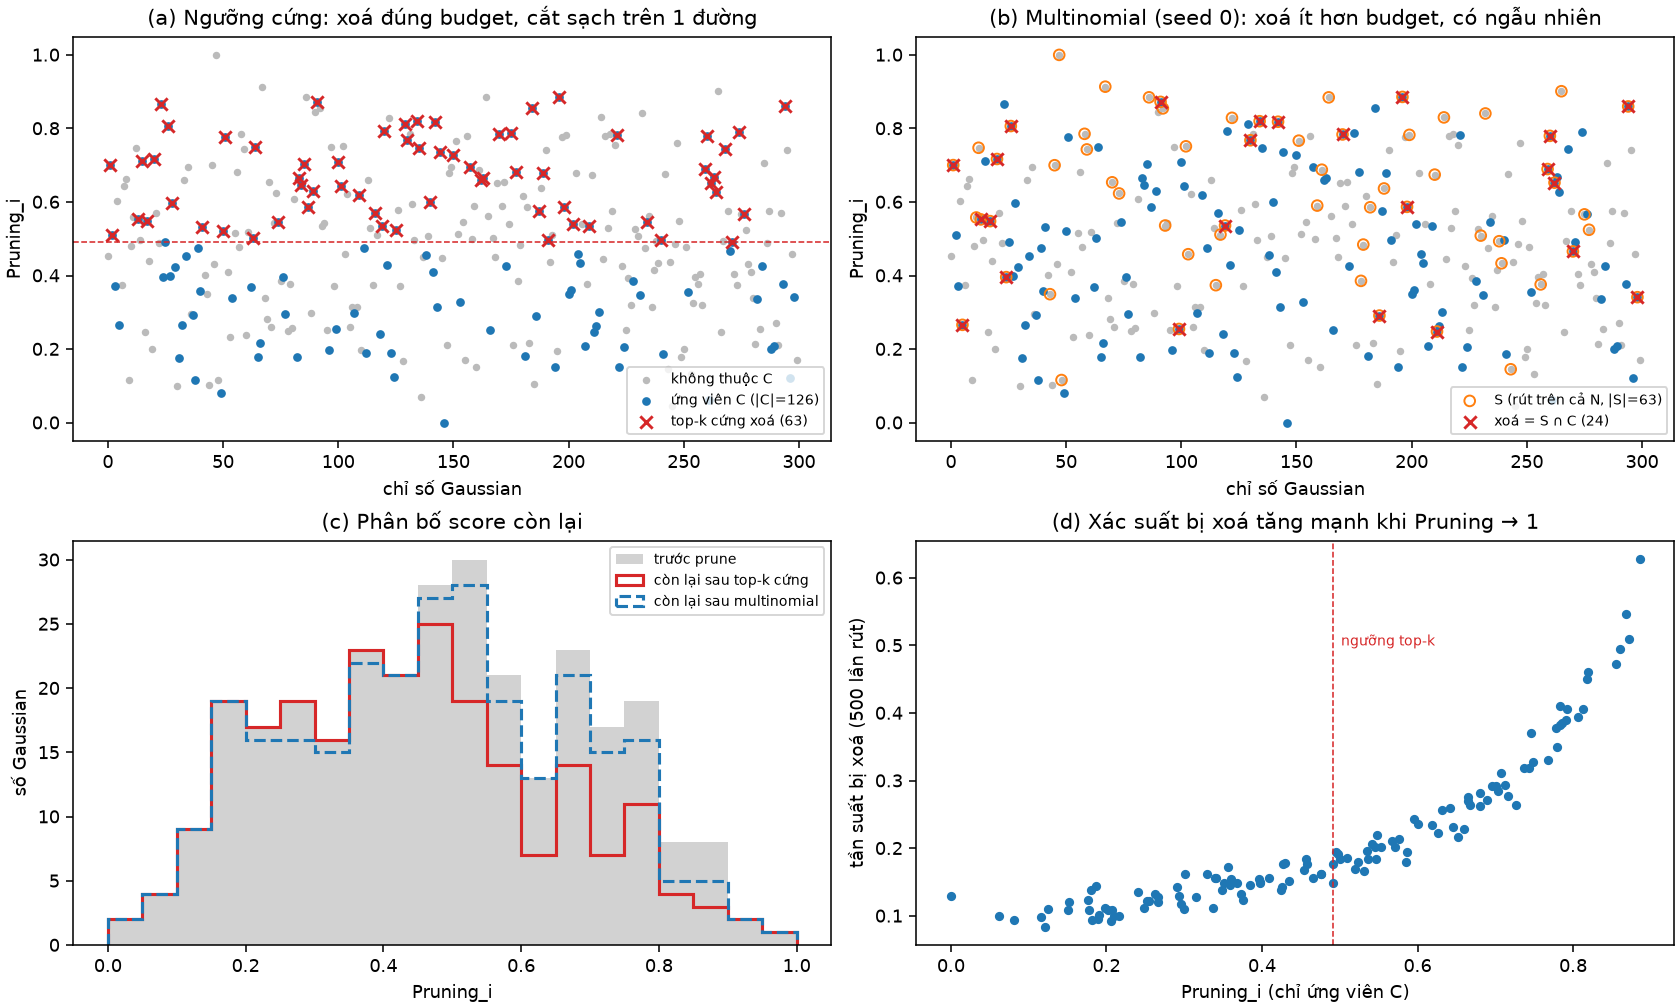
\includegraphics[width=0.95\linewidth]{5_3_topk-vs-multinomial.png}
\captionof{figure}{\footnotesize (a) top-k cứng cắt theo một đường ngưỡng; (b) multinomial xoá ít hơn budget, có ngẫu nhiên; (c) phân bố điểm còn lại; (d) xác suất bị xoá tăng mạnh khi $P_i\to 1$.}
\end{column}
\end{columns}
\end{frame}

% ===== Slide 26 (nguon: partADC_6.tex, frame "Toy model 2D: mục tiêu và một Gaussian") =====
\begin{frame}{Toy model 2D: mục tiêu và một Gaussian}
\begin{itemize}
    \footnotesize
    \item Ảnh mục tiêu $64\times 64$ px: hình tròn phẳng + vùng chi tiết (dải mảnh, chấm màu xen kẽ, ô vuông nhỏ).
    \item Mỗi Gaussian 2D: $G(x) = \exp\!\big(-\tfrac{1}{2}d^\top \Sigma^{-1} d\big)$, footprint giới hạn ở $3\sigma$.
    \item Render bằng alpha-compositing theo thứ tự chỉ số: $I(x) = \sum_i T_i\,\alpha_i G_i(x)\,c_i + T_{\text{end}}\cdot\text{bg}$, với $T_i = \prod_{j<i}(1-\alpha_j G_j)$.
\end{itemize}
\begin{center}
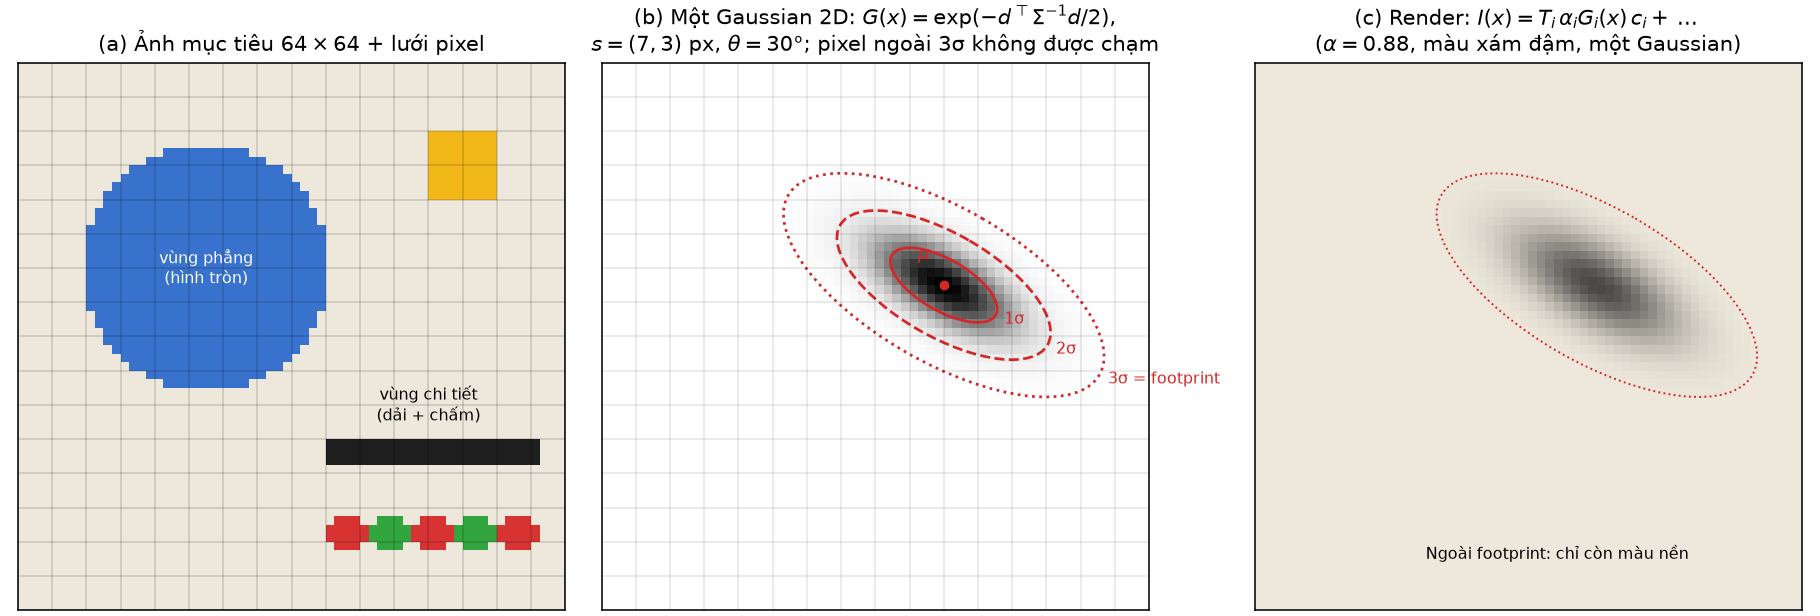
\includegraphics[width=0.75\linewidth]{6_1_muc-tieu-va-gaussian-2d.png}
\captionof{figure}{\footnotesize (a) Ảnh mục tiêu + lưới pixel; (b) một Gaussian $s=(7,3)$ px, $\theta=30°$ với các đường mức $1\sigma,2\sigma,3\sigma$; (c) kết quả render của Gaussian đó lên nền.}
\end{center}
\end{frame}

% ===== Slide 27 (nguon: partADC_6.tex, frame "So sánh trực tiếp: không ADC vs có ADC") =====
\begin{frame}{So sánh trực tiếp: không ADC vs có ADC}
\begin{columns}[T]
\begin{column}{0.5\textwidth}
\scriptsize
\begin{itemize}
    \item Ba kịch bản: (1) không ADC, $N{=}N_0$; (2) không ADC, khởi tạo ngẫu nhiên $N{=}N_{\text{cuối}}$; (3) có ADC, $N_0{\to}N_{\text{cuối}}$ dần.
    \item (2) cùng số Gaussian (3) nhưng khởi tạo ngẫu nhiên không khớp tự nhiên vào vùng chi tiết.
    \item[$\Rightarrow$] ADC không chỉ tăng $N$ mà đặt đúng chỗ cần thiết.
\end{itemize}
\end{column}
\begin{column}{0.5\textwidth}
\centering
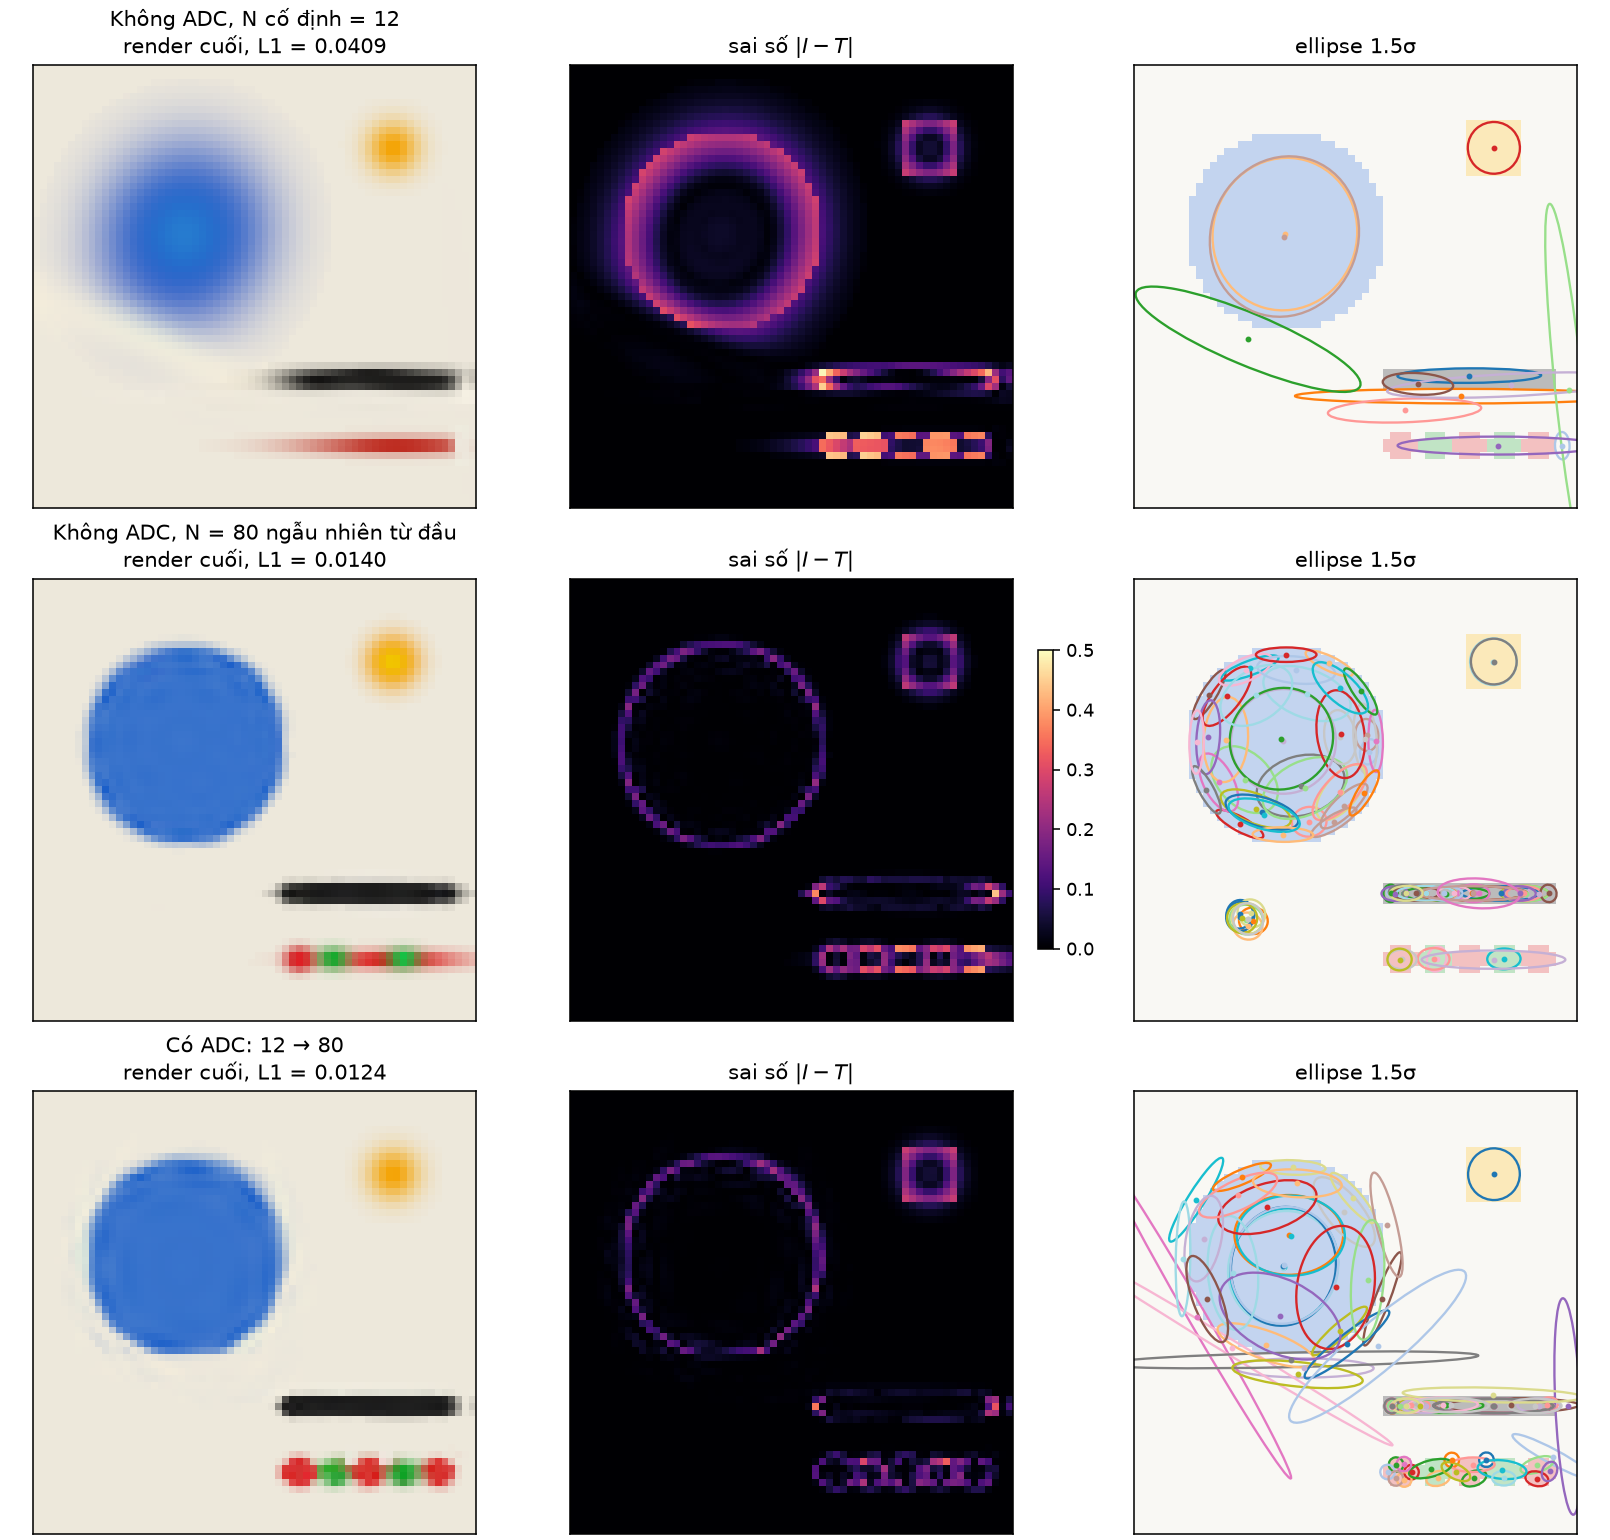
\includegraphics[width=0.85\linewidth]{6_10_khong-adc-vs-co-adc.png}
\captionof{figure}{\footnotesize 3 hàng (không ADC $N_0$; ngẫu nhiên; có ADC) $\times$ 3 cột.}
\end{column}
\end{columns}
\end{frame}

% ===== Slide 28 (nguon: partADC_7.tex, frame "Kết quả render cuối cùng: 3 kịch bản đối chiếu") =====
% KET QUA QUAN TRONG -- giu du noi dung.
\begin{frame}{Kết quả render cuối cùng: 3 kịch bản đối chiếu}
\scriptsize
\begin{itemize}
  \item Hàng 1 — \textbf{ADC 3DGS gốc}: $N$ tăng từ khởi tạo lên $N$ cuối, $L_1$ cuối như trong hình.
  \item Hàng 2 — \textbf{ADC FastGS-lite}: $L_1$ cuối \textbf{tương đương} nhưng \textbf{ít Gaussian hơn} — hiệu quả của Importance + prune multinomial + final prune.
  \item Hàng 3 — \textbf{Không ADC}: $N{=}N_0$ cố định, không clone/split/prune — chất lượng kém hơn rõ rệt.
  \item Mỗi hàng: render cuối, sai số $|I-T|$, ellipse $1.5\sigma$. Viền màu: đỏ=3DGS, xanh=FastGS, xám=không ADC.
\end{itemize}
\centering
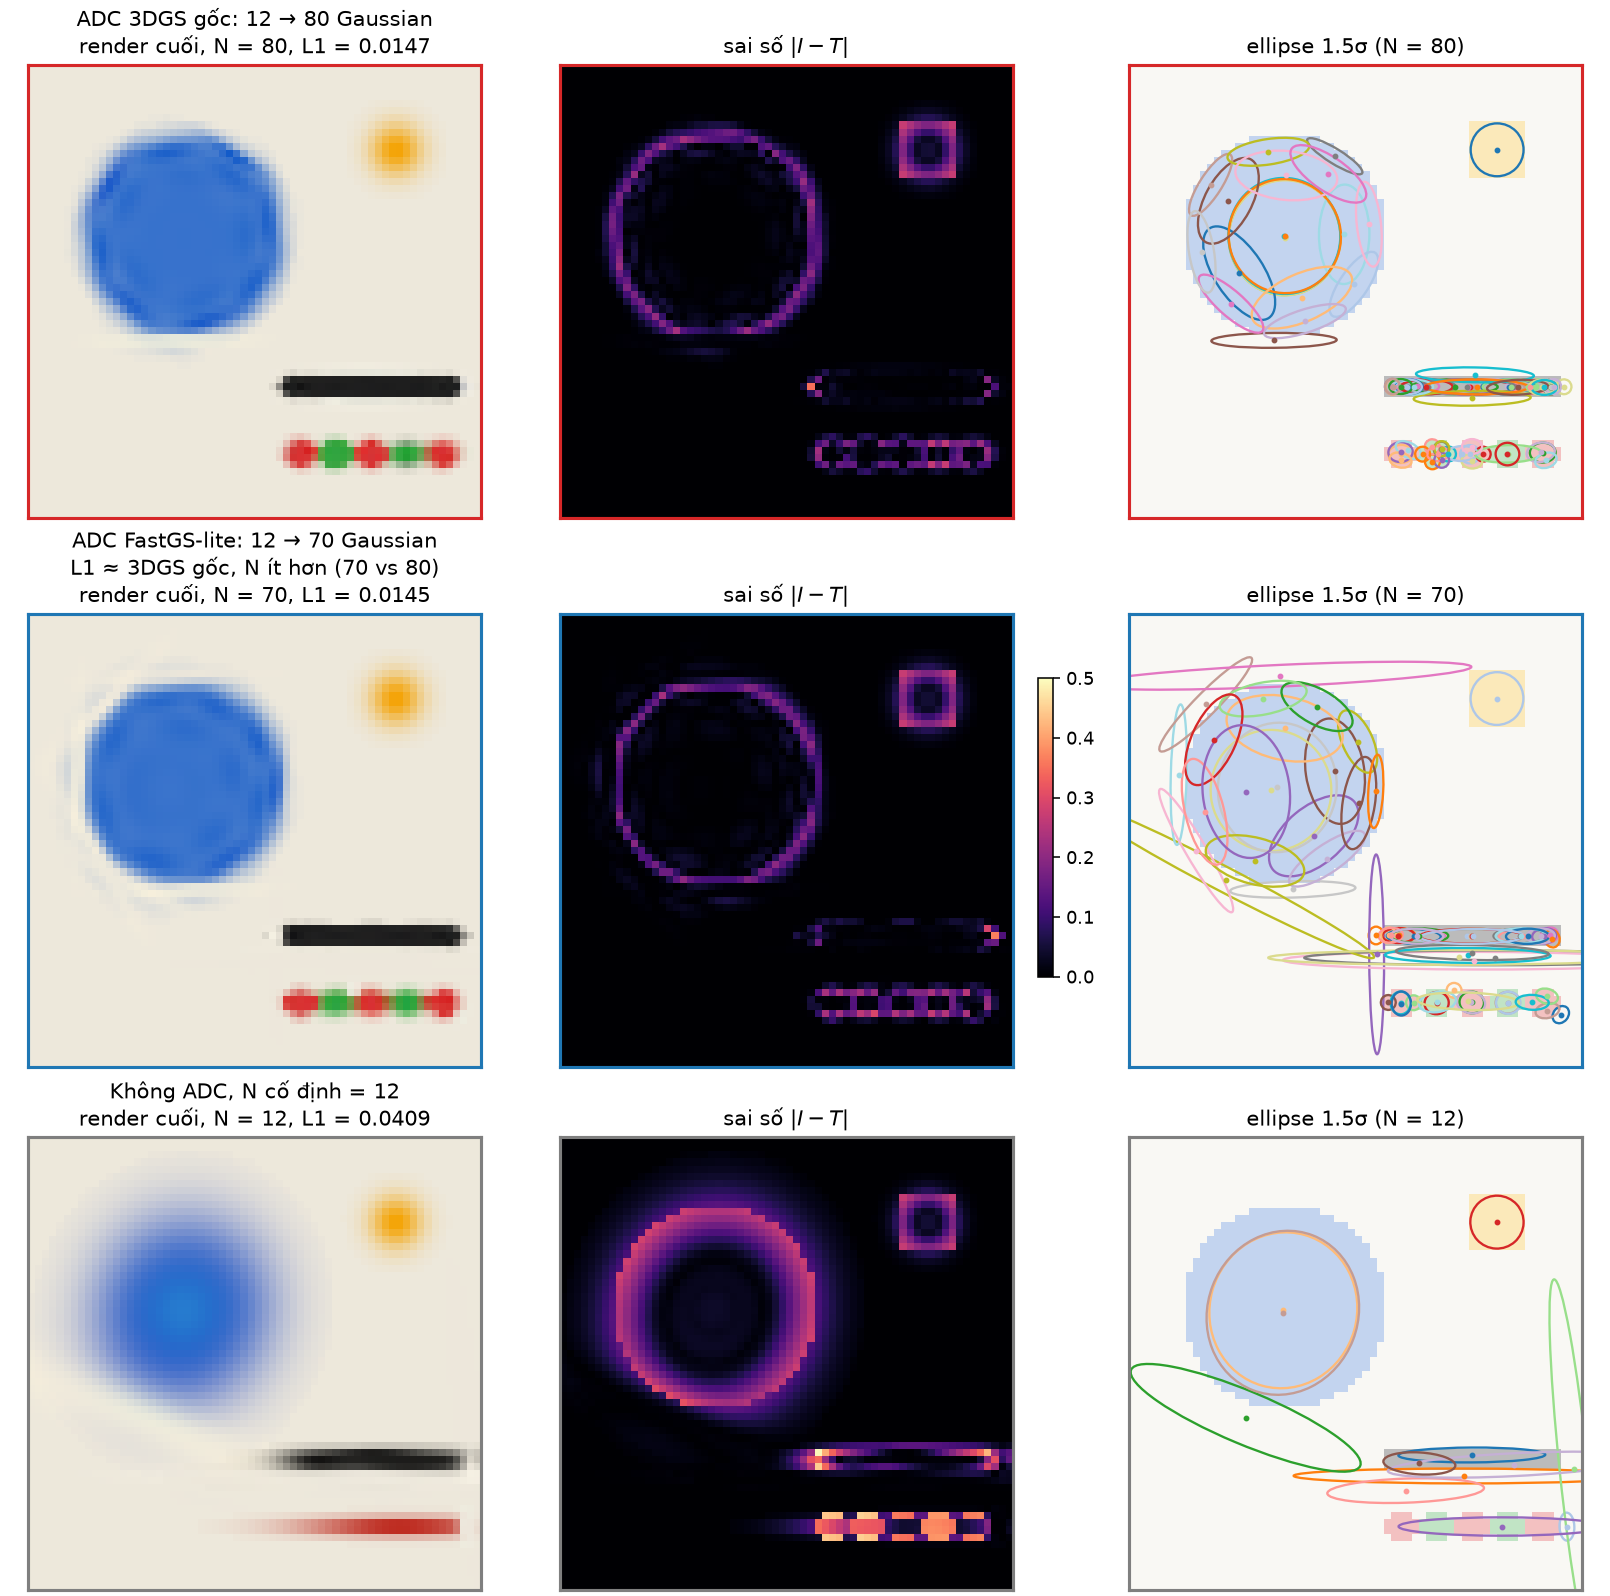
\includegraphics[width=0.42\linewidth]{7_5_cuoi-3dgs-fastgs-khong-adc.png}
\captionof{figure}{\footnotesize Đối chiếu cuối: ADC 3DGS gốc / ADC FastGS-lite / không ADC.}
\end{frame}

% ============================================================
% Bản 45 phút -- Slide 29-32
% Nguồn: partADC_7.tex (Slide 29) + part5.tex (Slide 30-32)
% CHỈ TẠO MỚI trong Slides45min/, không sửa file gốc.
% ============================================================

% --- Slide 29 (gốc: partADC_7.tex, "Cải tiến 5: final prune trên toy — khép lại chương ADC") ---
\begin{frame}{Tổng kết 5 cải tiến ADC của FastGS-lite}
\footnotesize
\begin{itemize}
  \item \textbf{5 cải tiến ADC}: (1) Importance đa view AND với gradient; (2) split theo gradient tuyệt đối; (3) prune multinomial; (4) trần opacity 0.8; (5) final prune sau densify.
\end{itemize}
\begin{columns}[T]
\begin{column}{0.52\textwidth}
\scriptsize
\begin{itemize}
  \item Final prune tại $t{\in}(1000,1100)$: $\text{rm}{=}[\alpha{<}0.1] \vee [\text{Pruning}{>}0.9]$.
  \item 3DGS gốc không có bước này -- $N(t)$ phẳng $[900,1200]$; FastGS giảm "hai bậc thang".
  \item Scatter $(\alpha,\text{Pruning})$: vùng "chữ L" bị xoá, đánh dấu X đỏ.
  \item[$\Rightarrow$] \textbf{Kết luận:} $L_1$ tương đương 3DGS gốc nhưng $N$ nhỏ hơn hẳn -- khép lại chương ADC, mở sang phần tăng tốc.
\end{itemize}
\end{column}
\begin{column}{0.48\textwidth}
\centering
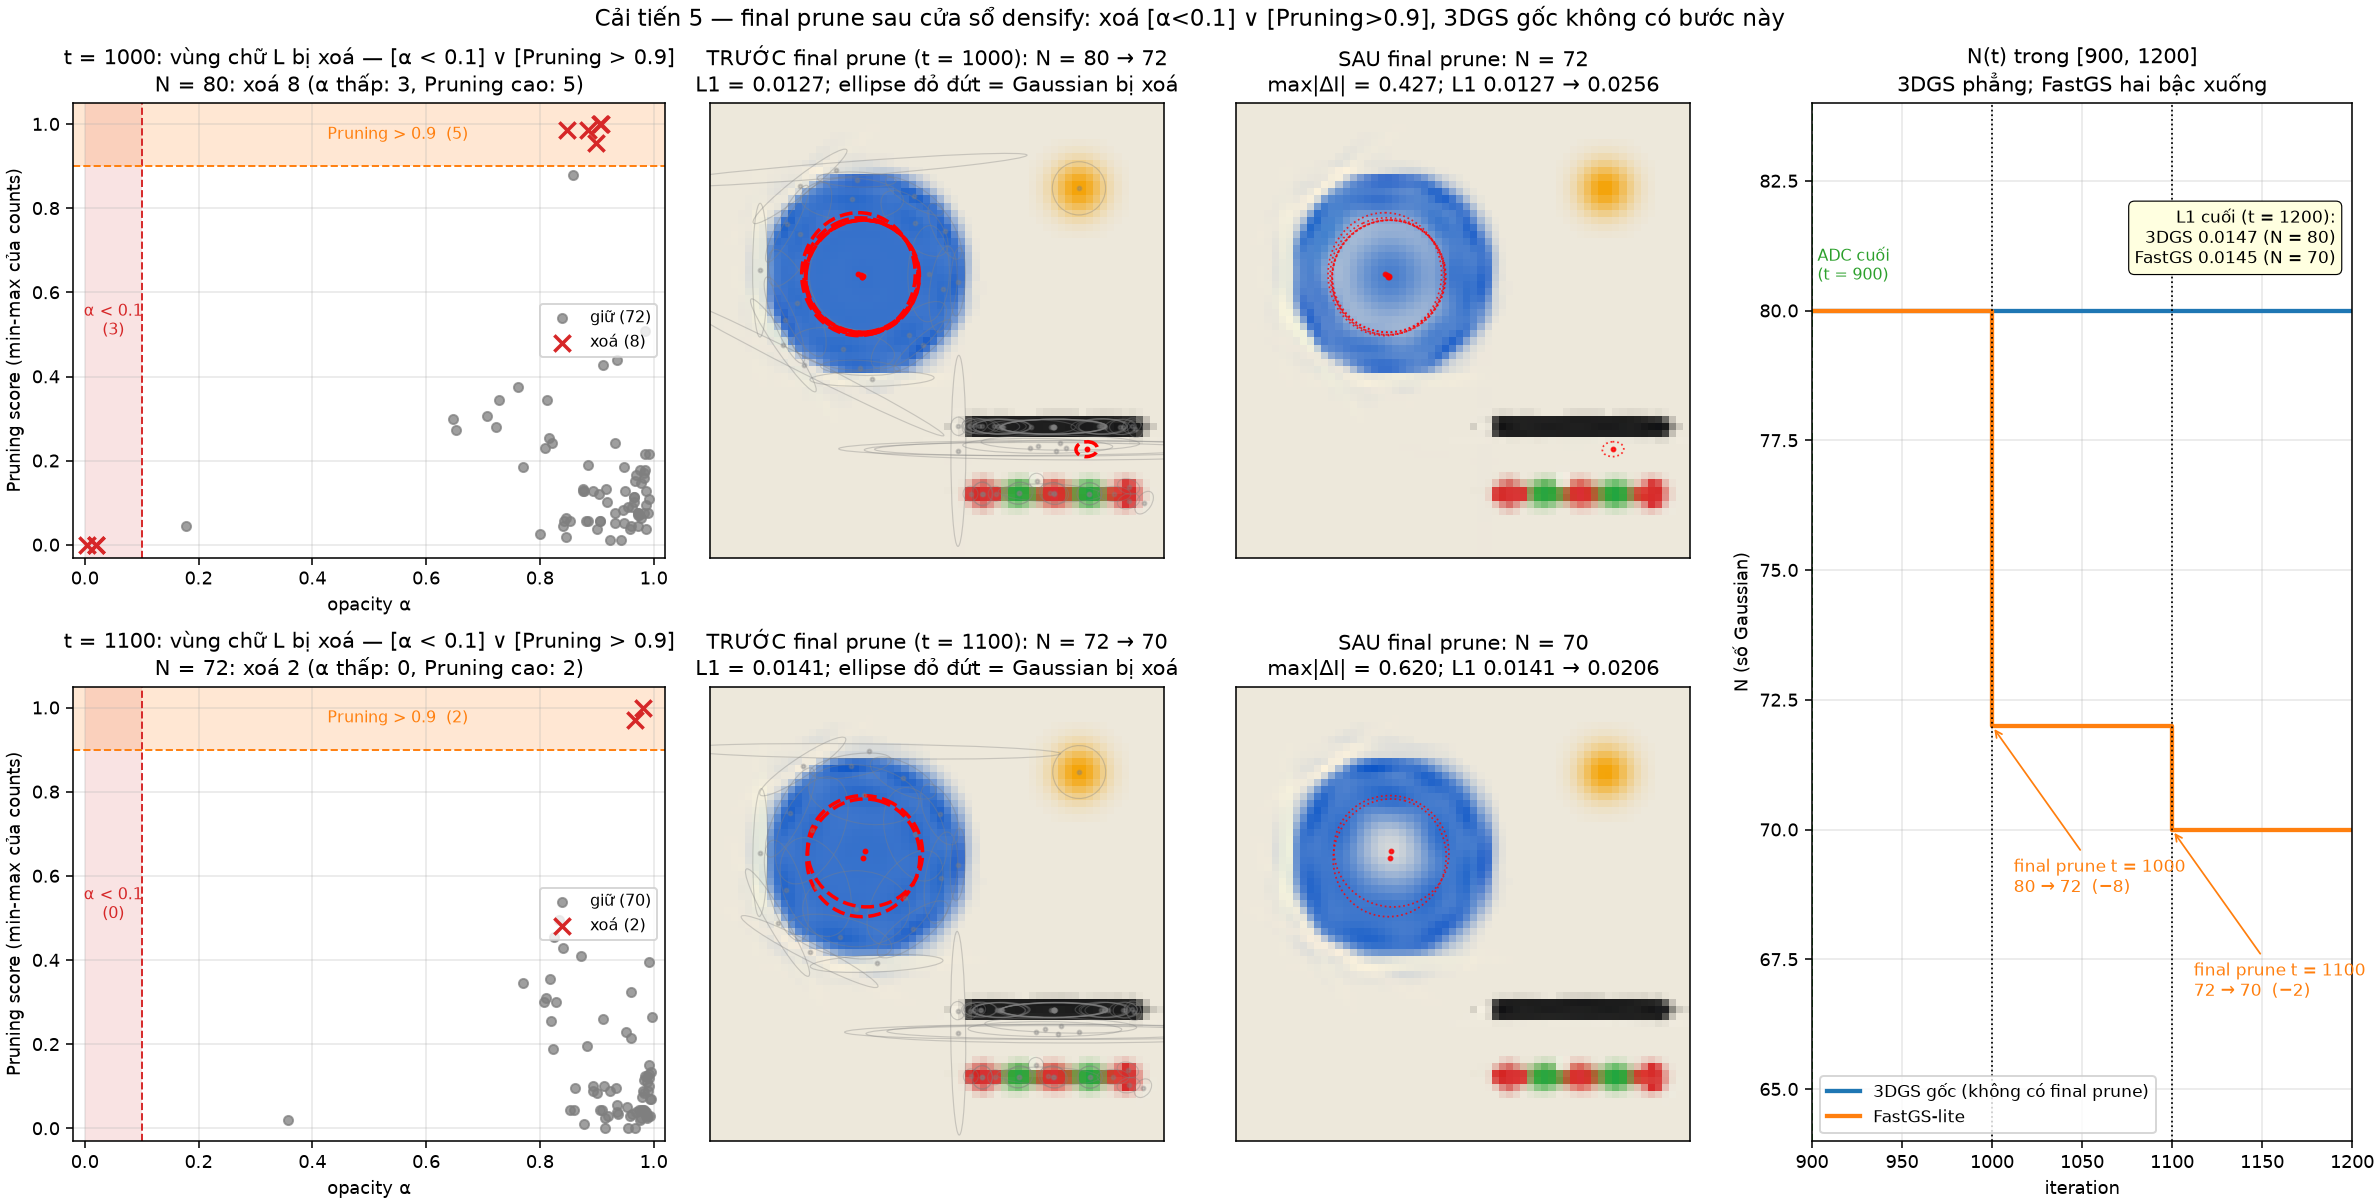
\includegraphics[width=0.95\linewidth]{7_10_final-prune-tren-toy.png}
\captionof{figure}{\footnotesize Final prune sau densify: xoá $[\alpha{<}0.1]\vee[\text{Pruning}{>}0.9]$.}
\end{column}
\end{columns}
\end{frame}

% --- Slide 30 (gốc: part5.tex, "Vì sao 3DGS gốc chậm?") ---
\begin{frame}{Vì sao 3DGS gốc chậm?}
\begin{itemize}
    \item Mỗi iteration gồm: \textbf{render} (rasterize), \textbf{tính loss}, \textbf{backward}, định kỳ \textbf{densify/prune}.
    \item Với hàng trăm nghìn -- hàng triệu Gaussian, \textbf{rasterize} và \textbf{backward} chiếm phần lớn thời gian mỗi bước.
\end{itemize}
\vspace{0.3cm}
\centering
\footnotesize
\begin{tabular}{lcc}
\toprule
\textbf{Khâu} & \textbf{Tần suất} & \textbf{Tỉ trọng thời gian} \\
\midrule
Render (project + rasterize) & mỗi iteration & \textasciitilde 45\% \\
Backward (gradient) & mỗi iteration & \textasciitilde 35\% \\
Tính loss & mỗi iteration & \textasciitilde 10\% \\
Densify/Prune & định kỳ & \textasciitilde 10\% (đột biến) \\
\bottomrule
\end{tabular}
\end{frame}

% --- Slide 31 (gốc: part5.tex, "Ba đòn bẩy tăng tốc của FastGS (tổng quan)") ---
\begin{frame}{Ba đòn bẩy tăng tốc của FastGS (tổng quan)}
\begin{columns}[t]
\column{0.33\linewidth}
\centering
\textbf{1. Multi-view score}
\begin{itemize}
    \footnotesize
    \item Đánh giá Gaussian qua nhiều góc nhìn
    \item Pruning thông minh hơn
\end{itemize}
\column{0.33\linewidth}
\centering
\textbf{2. Compact Box}
\begin{itemize}
    \footnotesize
    \item Giảm hệ số nhân bounding-box
    \item Giảm số tile chạm
\end{itemize}
\column{0.33\linewidth}
\centering
\textbf{3. Sparse Adam}
\begin{itemize}
    \footnotesize
    \item Lịch cập nhật phân tầng
    \item Giảm tần suất optimizer.step()
\end{itemize}
\end{columns}
\vspace{0.4cm}
\begin{itemize}
    \item Cả ba đòn bẩy nhắm đúng khâu chiếm tỉ trọng lớn nhất: rasterize, densify/prune, cập nhật tham số.
\end{itemize}
\end{frame}

% --- Slide 32 (gốc: part5.tex, "Hiệu năng tích luỹ: Biểu đồ thác nước") ---
\begin{frame}{Hiệu năng tích luỹ: Biểu đồ thác nước}
\footnotesize
\begin{itemize}
    \item Waterfall chart minh hoạ tăng tốc \textbf{tích luỹ} khi bật lần lượt từng đòn bẩy lên baseline 3DGS gốc.
    \item Thứ tự: baseline $\to$ + Compact Box $\to$ + Multi-view score $\to$ + Sparse Adam $\to$ FastGS đầy đủ.
\end{itemize}
\begin{center}
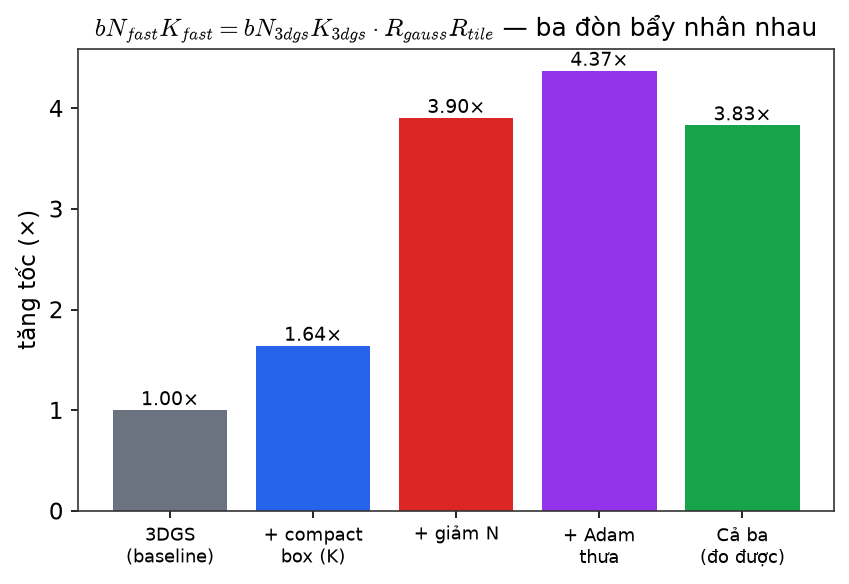
\includegraphics[width=0.68\linewidth]{ch8_levers_waterfall.png}
\end{center}
\end{frame}

% ============================================================
% PHẦN 9 (Slide 33--37, bản 45 phút): Tổng kết FastGS & kết quả FastGS-lite
% Rút gọn từ part5.tex (Slide "Tổng kết") và part6.tex (Slide 51, 55, 59, 60)
% ============================================================

% --- Slide 33 ---
\begin{frame}{Tổng kết: từ 3DGS gốc đến FastGS}
\centering
\footnotesize
\begin{tabular}{lll}
\toprule
\textbf{Tham số} & \textbf{3DGS gốc} & \textbf{FastGS} \\
\midrule
\texttt{loss\_thresh} & không có & mới, 0.1 \\
\texttt{grad\_abs\_thresh} & gradient thường & Abs-GS, 0.0012 \\
\texttt{--dense} & cố định & 0.001--0.013 (theo scene extent) \\
\texttt{--highfeature\_lr} & lr chuẩn & 0.005--0.02 (chia thêm /20) \\
\texttt{--mult} (box multiplier) & 3.0 & 0.5--0.7 \\
\bottomrule
\end{tabular}
\vspace{0.4cm}
\begin{itemize}
    \item FastGS không đổi mô hình biểu diễn cảnh, mà tối ưu \textbf{tham số hoá} và \textbf{lịch huấn luyện} dựa trên mô hình chi phí và định luật Amdahl $\Rightarrow$ tăng tốc mà PSNR/SSIM gần như không đổi.
\end{itemize}
\end{frame}

% --- Slide 34 ---
\begin{frame}{FastGS-lite: từ 24GB RTX 4090 xuống Colab T4 miễn phí}
\begin{itemize}
    \item \textbf{fastgs-lite}: fork giữ nguyên thuật toán FastGS gốc, chỉ đóng gói lại để chạy trên Colab T4 free tier -- không đổi công thức toán hay pipeline huấn luyện.
\end{itemize}
\vspace{0.3em}
\footnotesize
\begin{table}
\centering
\begin{tabular}{lll}
\toprule
\textbf{Tiêu chí} & \textbf{FastGS gốc} & \textbf{fastgs-lite} \\
\midrule
Phần cứng mục tiêu & 24GB RTX 4090 & T4 ($\sim$15GB VRAM) + 12.7GB RAM \\
CUDA extension & git submodule & vendor sẵn trong repo (\texttt{git clone}) \\
Entry point & train.py + shell script & train.py + notebook có instrumentation \\
Tín hiệu tiến trình & L1 + EMA & Score tổng hợp, log mỗi 1000 iter \\
\bottomrule
\end{tabular}
\end{table}
\end{frame}

% --- Slide 35 ---
\begin{frame}{Bảng 1: Chất lượng cuối cùng theo scene}
\footnotesize
\begin{table}
\centering
\begin{tabular}{lccccc}
\toprule
\textbf{Scene} & \textbf{Score} & \textbf{PSNR (dB)} & \textbf{SSIM} & \textbf{LPIPS} & \textbf{\#Gaussian} \\
\midrule
playroom  & 0.8198 & -- & -- & -- & $\sim$129k \\
drjohnson & 0.8027 & 27.41 & -- & -- & $\sim$174k \\
truck     & 0.7482 & -- & -- & -- & $\sim$187k \\
train     & 0.6867 & 19.75 & -- & -- & $\sim$201k \\
\midrule
\textbf{Mean} & \textbf{0.7643} & \textbf{24.46} & & & \\
\bottomrule
\end{tabular}
\end{table}
\begin{itemize}
    \item 2 scene indoor vượt 2 scene outdoor dù dùng \textbf{ít Gaussian hơn} (129k--174k so với 187k--201k).
\end{itemize}
\centering
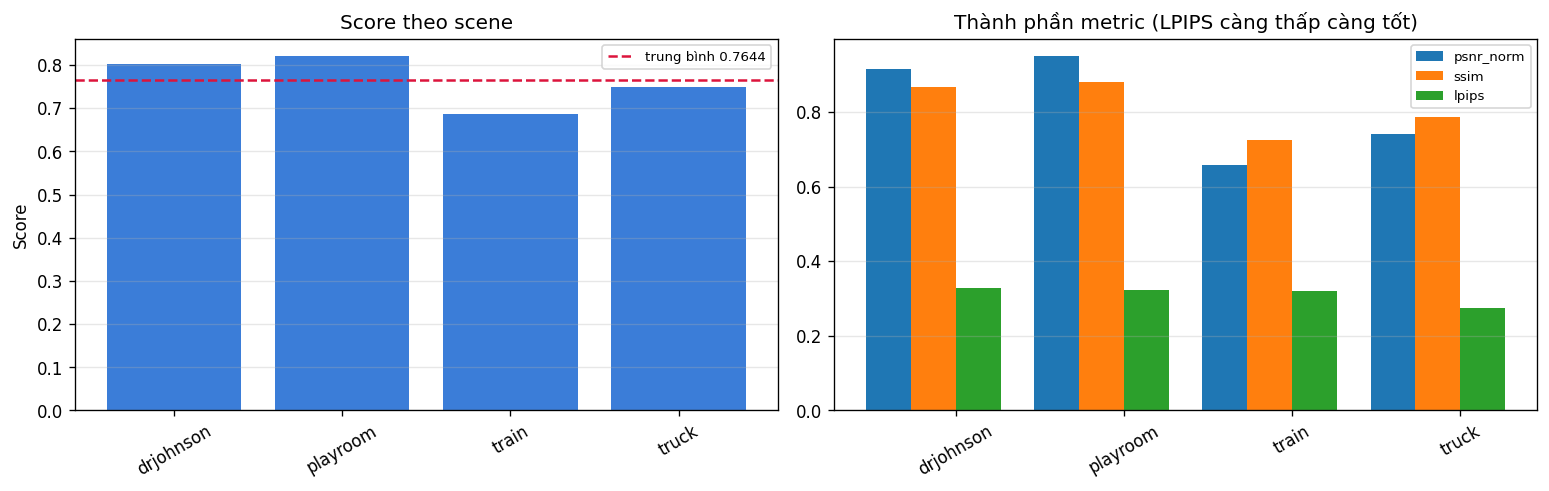
\includegraphics[width=0.5\linewidth]{leaderboard.png}
\captionof{figure}{Leaderboard Score theo scene}
\end{frame}

% --- Slide 36 ---
\begin{frame}{Bảng 3: Chi phí \& lưu trữ}
\begin{itemize}
    \item Tổng train 4 scene: \textbf{327.6s} ($\sim$5.5 phút), \textbf{85.5 iter/s} trung bình, VRAM đỉnh chỉ \textbf{0.88GB} (max 1.16GB).
    \item \texttt{.ply} trung bình \textbf{171.6MB}, đúng \textbf{248 byte/Gaussian} = record 3DGS không nén.
\end{itemize}
\vspace{0.3em}
\footnotesize
\centering
\begin{tabular}{lcc}
\toprule
\textbf{Chỉ số} & \textbf{Trung bình} & \textbf{Ghi chú} \\
\midrule
Thời gian train (4 scene) & 327.6 s & $\sim$5.5 phút tổng \\
Tốc độ & 85.5 iter/s & \\
VRAM peak & 0.88 GB & max 1.16GB (drjohnson) \\
Kích thước .ply & 171.6 MB & 248 byte/Gaussian \\
\bottomrule
\end{tabular}
\end{frame}

% --- Slide 37 ---
\begin{frame}{Khả năng tái lập \& giới hạn phép đo}
\footnotesize
\texttt{Config(resolution=2, iterations=7000, score\_every=1000,\\
\hspace{2em}eval\_views=6, psnr\_max=30.0, submission\_resolution=1)}
\normalsize
\vspace{0.5em}
\begin{itemize}
    \item \textbf{Giới hạn}: chạy \textbf{một lần duy nhất} (không seed/lặp lại), chỉ \textbf{4 scene} từ 2 dataset, ngân sách 7k iteration chỉ bằng \textbf{1/3} lịch 30k thiết kế gốc, bỏ qua bước prune cuối (\texttt{final\_prune\_fastgs}).
    \item[$\Rightarrow$] \textbf{Kết luận}: Bảng 1 là \emph{baseline có thể tái lập của repo này}, \textbf{không phải} benchmark chính thức để so sánh với FastGS/3DGS gốc.
\end{itemize}
\end{frame}

% ============================================================
% PHẦN Faster-GS (bản 45 phút, rút gọn) — 2 slide
% Rút gọn từ part_fastergs_01.tex..08.tex (bản full, ../part_fastergs_*.tex)
% ============================================================

% --- Slide A ---
\begin{frame}{Faster-GS (CVPR 2026): 4 cơ chế mới luôn bật}
\footnotesize
\begin{itemize}
    \item \textbf{Fused Adam}: 1 kernel CUDA elementwise, đúng công thức Adam chuẩn (không đổi thuật toán, chỉ giảm overhead kernel-launch).
    \item \textbf{3D anti-aliasing filter}: clamp scale tối thiểu theo khoảng cách camera $\Rightarrow$ chống alias.
    \item \textbf{Morton Z-order reordering}: sắp Gaussian theo mã bit-interleave (mỗi 5000 iteration) $\Rightarrow$ tăng cache locality cho rasterizer.
    \item \textbf{Random-init fallback}: sample đều trong hình cầu bằng $r=R\cdot u^{1/3}$ khi COLMAP thiếu \texttt{points3D}.
    \item[$\Rightarrow$] Cả 4 đều \textbf{luôn bật}, không còn cờ toggle.
    \item \textit{Ngoại lệ}: MCMC densification có sẵn trong code nhưng \textbf{giữ tắt} — xung đột kiến trúc với densify chính của FastGS.
\end{itemize}
\centering
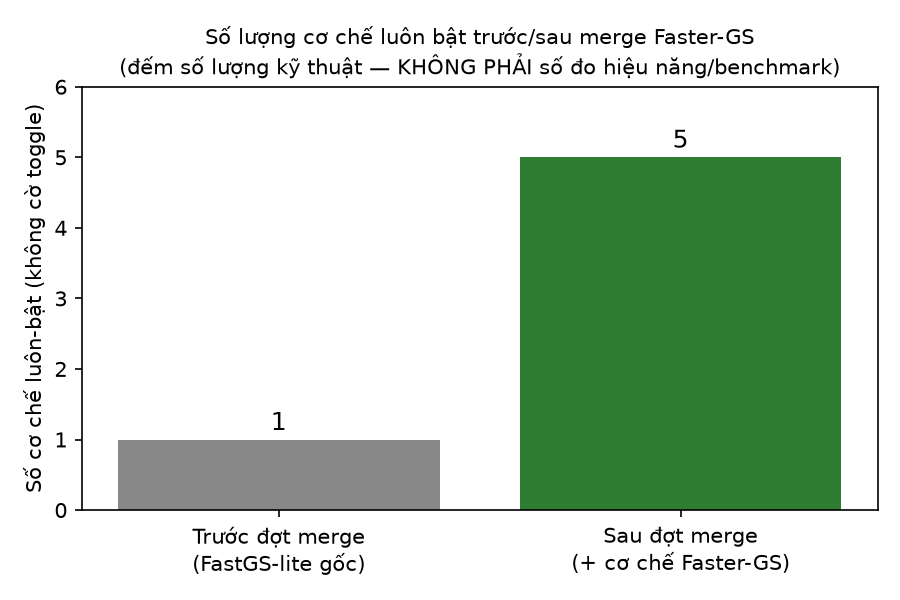
\includegraphics[width=0.3\linewidth]{../../BOOK/fastergs_merge_figures/00_techniques_overview.png}
\captionof{figure}{\footnotesize Số cơ chế luôn bật trước/sau đợt merge (đếm số lượng, không phải benchmark)}
\end{frame}

% --- Slide B ---
\begin{frame}{Bug đã sửa: \texttt{opacity\_reset\_interval} không co giãn theo iterations}
\footnotesize
\begin{itemize}
    \item \textbf{Nguyên nhân thật} của các điểm sụt Score đã thấy (Slide 33--37): \texttt{opacity\_reset\_interval} hardcode \textbf{3000} (đúng cho lịch gốc 30k), \textbf{không co giãn} theo \texttt{iterations} đã rút ngắn $\Rightarrow$ reset kích hoạt quá sớm.
    \item Bằng chứng thật: PSNR rơi \textbf{22.02$\to$5.92} tại iteration 3000 (scene HCM0539).
    \item \textbf{Cách sửa}: field mới \texttt{opacity\_reset\_frac=0.2}, co giãn \texttt{opacity\_reset\_interval = round(0.2$\times$iterations)}.
    \item Chưa có log thật "sau khi sửa" — chưa build/chạy lại (không có GPU ở môi trường phát triển).
\end{itemize}
\centering
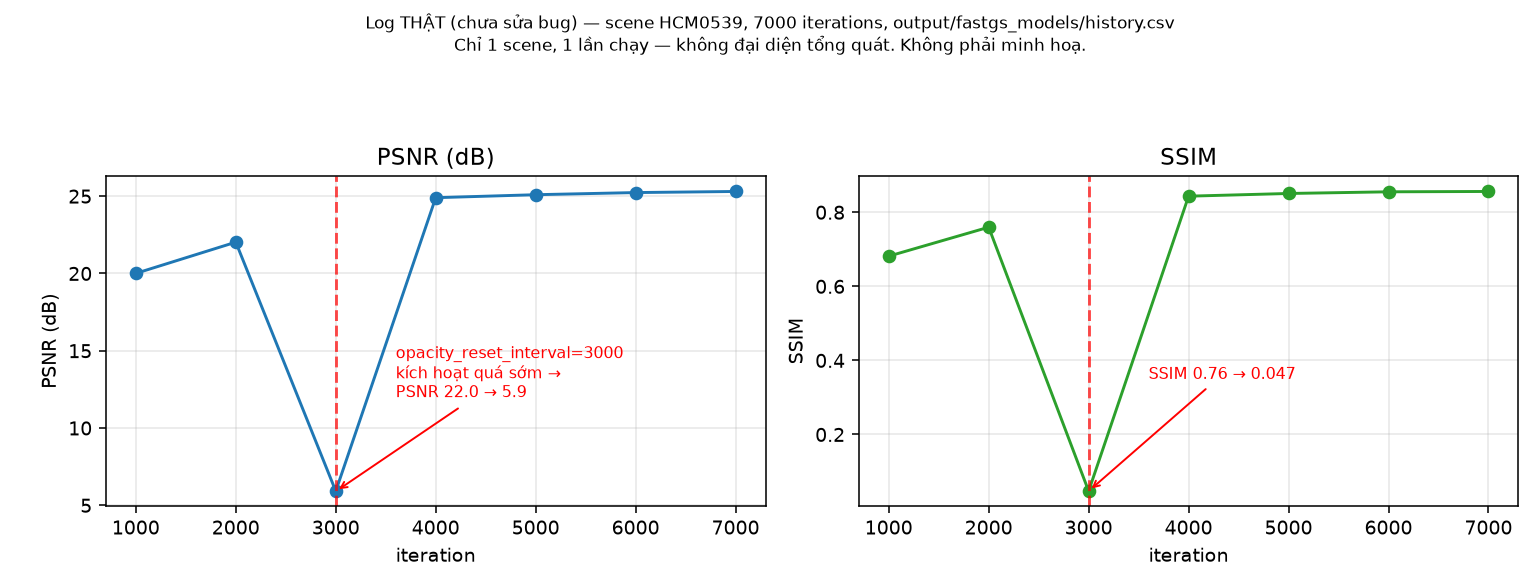
\includegraphics[width=0.32\linewidth]{../../BOOK/adc_figures/12_opacity_reset_crash_real_log.png}
\captionof{figure}{\footnotesize Log thật (trước khi sửa): PSNR sụp tại iteration 3000}
\end{frame}

% ============================================================
% PHẦN 45 phút — Slide 38-41 (Quan sát RAM, Tổng kết pipeline,
% Tổng kết FastGS & giới hạn, Cảm ơn / Q&A) — rút gọn từ part7.tex
% ============================================================

% --- Slide 38 (gốc: Slide 62 — Quan sát 2) ---
\begin{frame}{Quan sát 2: Nút thắt là RAM hệ thống, không phải VRAM}
\begin{itemize}
    \item Đo trên Google Colab T4 trong quá trình huấn luyện:
\end{itemize}
\footnotesize
\begin{table}[]
\centering
\begin{tabular}{lccc}
\toprule
Tài nguyên & Đỉnh sử dụng & Khả dụng & \% sử dụng \\
\midrule
VRAM (GPU) & 1.16 GB & 14.56 GB & \textbf{8\%} \\
RAM hệ thống & 9.59 GB & 12.7 GB & \textbf{91\%} (giới hạn mềm 10.5 GB) \\
\bottomrule
\end{tabular}
\end{table}
\normalsize
\begin{itemize}
    \item RAM hệ thống áp sát giới hạn mềm, trong khi VRAM còn dư rất nhiều.
    \item Khuyến nghị cũ "giảm độ phân giải để tiết kiệm VRAM" \textbf{không cần thiết} ở ngân sách này.
\end{itemize}
\end{frame}

% --- Slide 39 (gốc: Slide 64 — Tổng kết pipeline) ---
\begin{frame}{Tổng kết pipeline render 3D Gaussian Splatting}
\centering
\footnotesize
\begin{tikzpicture}[
    node distance=8mm and 6mm,
    box/.style={draw, rounded corners, align=center, minimum height=0.9cm, minimum width=2.6cm, fill=blue!8}
]
\node[box] (gauss) {3D Gaussian\\$(\mu,\Sigma,\alpha,SH)$};
\node[box, right=of gauss] (proj) {Chiếu phối cảnh\\(EWA)};
\node[box, right=of proj] (raster) {Rasterizer khả vi\\theo tile};

\node[box, below=of raster] (blend) {Alpha\\blending};
\node[box, left=of blend] (loss) {Loss\\($L_1$+D-SSIM)};
\node[box, left=of loss] (back) {Backward\\(gradient)};

\node[box, below=of back, fill=orange!12] (adc) {Adaptive\\Density Control};

\draw[-Latex] (gauss) -- (proj);
\draw[-Latex] (proj) -- (raster);
\draw[-Latex] (raster) -- (blend);
\draw[-Latex] (blend) -- (loss);
\draw[-Latex] (loss) -- (back);
\draw[-Latex] (back) -- (adc);
\draw[-Latex] (adc) -- (gauss);
\end{tikzpicture}
\vspace{2mm}

\normalsize
Một chu trình khép kín: render $\rightarrow$ tính loss $\rightarrow$ lan truyền ngược $\rightarrow$ điều chỉnh mật độ Gaussian $\rightarrow$ lặp lại.
\end{frame}

% --- Slide 40 (gốc: Slide 65 — Tổng kết cải tiến FastGS \& giới hạn) ---
\begin{frame}{Tổng kết cải tiến FastGS \& giới hạn còn lại}
\textbf{Ba đòn bẩy chính:}
\begin{itemize}
    \item \textbf{Multi-view score} + \textbf{Compact box} $\Rightarrow$ giảm Gaussian dư thừa mà không giảm chất lượng đáng kể.
    \item \textbf{Sparse Adam} $\Rightarrow$ giảm chi phí tính toán mỗi iteration.
\end{itemize}
\vspace{2mm}
\textbf{Giới hạn / hướng phát triển:}
\begin{enumerate}
    \item Dữ liệu Gaussian đầu ra chưa được nén (248 B/Gaussian, thô).
    \item Ngân sách 7k iteration bỏ lỡ bước \texttt{final\_prune}.
    \item Chưa có ablation study cô lập riêng từng đòn bẩy.
    \item 4 nhánh mở rộng của FastGS gốc — dynamic scenes, sparse view, surface reconstruction, SLAM — chưa tích hợp vào fork này.
\end{enumerate}
\end{frame}

% --- Slide 41 (gốc: Slide 67 — Cảm ơn / Q&A, frame cuối cùng) ---
\begin{frame}[c]{}
\centering
{\Huge \textbf{Cảm ơn đã theo dõi!}}

\vspace{6mm}
{\LARGE Hỏi đáp (Q\&A)}

\vspace{10mm}
{\small Digital Twin GS --- FastGS-lite \\ \texttt{github.com/KietAnhCS/fastgs-lite}}
\end{frame}


\end{document}
